\documentclass[a4paper,hidelinks,12pt]{article}
% \usepackage{geometry}
\usepackage{amsmath,graphicx}
\usepackage[utf8]{inputenc}
\usepackage[russian]{babel}
\usepackage{indentfirst}
\usepackage{colortbl}
\usepackage{setspace}
\usepackage{float}
\usepackage[noend]{algorithmic}
\usepackage[nottoc,notlot,notlof]{tocbibind}
\usepackage{amssymb}
\usepackage{amsmath}
\usepackage{graphicx}
\usepackage{listings}
\usepackage{subcaption}
\usepackage[boxruled]{algorithm2e}
\usepackage{setspace}
\usepackage{natbib}
\usepackage{minted}
\usepackage{subcaption}
    
\SetKwInput{KwData}{Входные данные}
\SetKwInput{KwResult}{Результат}

\SetKwIF{If}{ElseIf}{Else}{если}{тогда}{иначе если}{иначе}{конец если}
\SetKwFor{For}{для}{сделать}{конец для}

\SetKw{Return}{вернуть}
\SetKw{End}{конец}
\SetKw{KwIn}{в}

\usepackage{xcolor}
\definecolor{gray}{rgb}{0.4,0.4,0.4}
\definecolor{darkblue}{rgb}{0.0,0.0,0.6}
\definecolor{cyan}{rgb}{0.0,0.5,0.5}
\definecolor{maroon}{rgb}{0.5,0,0}
\definecolor{darkgreen}{rgb}{0,0.5,0}

\usepackage[left=3cm,right=2cm,top=2cm,bottom=2cm,bindingoffset=0cm]{geometry}
\setcounter{secnumdepth}{4}
% \linespread{1.6}
\setlength{\baselineskip}{1.6}
\usepackage{xcolor}
\usepackage{pdfcomment}

\newcommand{\todo}[1]{\textcolor{red}{\texttt{#1}}}

\usepackage{wrapfig}
\usepackage{graphicx}
\graphicspath{ {./pictures/} }

\everymath{\displaystyle}

% \tolerance=1
% \emergencystretch=\maxdimen
% \hyphenpenalty=10000
% \hbadness=10000

\begin {document}
\begin {titlepage}
\thispagestyle{empty}

\begin{center}
\vspace{-1cm}

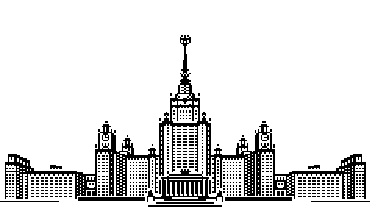
\includegraphics[width=0.5\textwidth]{msu}\\
Московский Государственный Университет им. М.В. Ломоносова\\
Факультет Вычислительной Математики и Кибернетики\\

\vspace{3cm}

{\Large Кожевников Евгений Владимирович}

\vspace{1cm}

% par made the trick here idk why
{\LARGE\bfseries Отчёт заданию №3 в рамках курса <<Суперкомпьютерное моделирование\\ и технологии>>\par}

\vspace{1cm}

{\Large\bfseries Вариант 8}

\end{center}

\vfill

\begin{center}
Москва, 2023
\end{center}

\end{titlepage}

\setcounter{page}{2}
\onehalfspacing

\newpage
\tableofcontents

\setlength{\parskip}{0.8em}
\newpage

\section{Постановка задачи}

Рассматривается дифференциальная задача для для трёхмерного гиперболического уравнения в области, представляющей из себя прямоугольный параллелепипед.

В трёхмерной замкнутой области
% 
\[ \Omega  = [0 \leqslant x \leqslant L_x] \times [0 \leqslant y \leqslant L_y] \times [0 \leqslant z \leqslant L_z] \]
% 
\noindent для \( 0 < t \leqslant T \) требуется найти решение \( u(x,y,z,t) \) уравнения в частных производных
% 
\[ \frac{\partial ^ 2 u}{\partial t ^ 2} = a ^ 2 \Delta u \]
% 
\noindent с начальными условиями
% 
\begin{align*}
u |_{t=0} &= \varphi (x, y, z) \\
\left.\frac{\partial u}{\partial t}\right|_{t=0} &= 0
\end{align*}
% 
\noindent при условии, что на границе области заданы периодические граничные условия
% 
\begin{align*}
    u(0, y, z, t) &= u(L_x, y, z, t) & u_x(0, y, z, t) &= u_x(L_x, y, z, t) \\
    u(x, 0, z, t) &= u(x, L_y, z, t) & u_y(x, 0, z, t) &= u_y(x, L_y, z, t) \\
    u(x, y, 0, t) &= u(x, y, L_z, t) & u_z(x, y, 0, t) &= u_y(x, y, L_z, t) \\
\end{align*}

В соответствии с \textbf{вариантом 8}, аналитическое решение задано следующим образом:
% 
\begin{align*}
    u_{analytical} &= \sin{\left( \frac{2\pi}{L_x} x \right)}
        \cdot \sin{\left( \frac{4\pi}{L_y}y \right)}
        \cdot \sin{\left( \frac{6\pi}{L_z} z \right)}
        \cdot \cos{\left( a_t \cdot t \right)} \\
    a_t &= \sqrt{\frac{4}{L_x^2} + \frac{16}{L_y^2} + \frac{36}{L_z^2}} \\
    a^2 &= 1
\end{align*}

\newpage

\section{Численный метод решения задачи}

Введём на \( \Omega \) сетку \( \omega_{h\tau} = \overline{\omega}_h \times \omega_\tau \). Через \( \omega_h \) обозначим множество внутренних, а через \( \gamma_h \) --- множество граничных узлов сетки \( \overline{\omega}_h \).

Через $\Delta_h$ обозначим семиточечный разностный аналог оператора Лапласа.

Для начала счёта определим значения \( u \) для первых двух итераций:
% 
\begin{align*}
    u^0_{ijk} &= \varphi (x_i, y_j, z_k) \in \overline{\omega_h} \\
    u^1_{ijk} &=
      \begin{cases}
      u^0_{ijk} + a^2\frac{\tau^2}{2}\Delta_h\varphi(x_i,y_j,z_k), & (x_i, y_j, z_k) \in \omega_h \\
      u_{analytical}(x_i, y_j, z_k, \tau), & (x_i, y_j, z_k) \in \gamma_h
    \end{cases}
\end{align*}

Из явной разностной схемы 

\[ \frac{u^{n+1}_{ijk} - 2u^n_{ijk} + u^{n-1}_{ijk}}{ \tau^2} = a^2 \Delta_h u^n,\quad (x_i, y_j, z_k) \in \omega_h \]

\noindent выразим значения $u^{n+1}_{ijk}$ на $(n+1)$-м шаге через значения на предыдущих слоях:

\[ u^{n+1}_{ijk} = 2u^n_{ijk} - u^{n-1}_{ijk} + \tau^2 a^2 \Delta_h u^n \]

\section{Программная реализация алгоритма с использованием технологий OpenMP и MPI}

В соответствии с заданием используется блочное разбиение. Для достижения наибольшей производительности выбраны фиксированные варианты разбиения пространства на блоки в зависимости от числа MPI процессов:

\begin{table}[H]
\centering
\begin{tabular}{|p{2cm}|p{2cm}|p{2cm}|p{2cm}|}
    \hline
    \textit{Число MPI процессов} & \textit{Число блоков по X} & \textit{Число блоков по Y} & \textit{Число блоков по Z} \\
    \hline
    1 & 1 & 1 & 1 \\
    2 & 2 & 1 & 1 \\
    4 & 2 & 2 & 1 \\
    8 & 2 & 2 & 2 \\
    16 & 2 & 2 & 4 \\
    32 & 2 & 4 & 4 \\
    \hline
\end{tabular}
\end{table}

Для получения блока в разбиении и создания топологии используется \texttt{MPI\_Comm\_Cart}.

Аналогично OpenMP и однопоточной реализации, для расчётов используются 3 массива, соответствующие текущему, предыдущему и пред-предыдущему моменту времени. Каждый блок разбиения использует свою тройку таких массивов.

В \textbf{варианте 8} периодические граничные условия по всем 3 осям. Они реализуются тем же механизмом, с помощью которого блоки передают свои внешние грани следующим блокам в топологии, с точностью до замыкания координат на 4-х мерном торе.

Для распараллеливания внутреннего цикла численного решения задачи каждый блок независимо использует \texttt{\#pragma omp parallel for collapse(N)}.

\section{Результаты запусков на IBM Polus}

Для компиляции использовался компилятор IBM \texttt{mpixlC} из модуля \texttt{SpectrumMPI}. В силу перебоев в работе гибридных программ на СК Polus, были произведены замеры с и без использования OpenMP.
% 
\begin{minted}[linenos=false]{bash}
# mpi+openmp
mpixlC v8.cpp -std=c++14 -DL=1 -DN=128 -DUSE_OMP -qsmp=omp -o v8
# mpi
mpixlC v8.cpp -std=c++14 -DL=1 -DN=128-o v8
\end{minted}

Для запуска использовалась утилита \texttt{mpisubmit.pl}:
% 
\begin{minted}[linenos=false]{bash}
# mpi+openmp
mpisubmit.pl -p N -t M ./v8
# mpi
mpisubmit.pl -p N ./v8
\end{minted}
% 
\noindent где M  --- число OpenMP нитей, с которым запустится программа, а N --- число MPI процессов.
% 

Ускорение $S$ и погрешность $\delta$ вычислялись следующим образом:
\begin{align*}
    S &= \frac{T|_{n threads, nprocesses}}{T|_{n threads = min, nprocesses=min}} \\
    \delta &= \sum_{(x_i, y_j, z_k) \in \omega_h} \left| u_{analytical}(x_i, y_j, z_k, T) - u_{calculated}(x_i, y_j, z_k, T) \right|
\end{align*}

Рассматривалось $K=20$ эпох симуляции от $T=0$ до $T=0.0001$. В итоговых таблицах представлено значение погрешности $\delta$ на заключительной эпохе симуляции.

\subsection{L = 1}

{
\centering
\noindent\begin{tabular}{|p{2cm}|p{2cm}|p{2.5cm}|p{2.5cm}|p{2cm}|p{2.5cm}|}
    \hline
    \textit{Число MPI процессов }$N_p$ & \textit{Число OpenMP нитей} & \textit{Число точек сетки }$N^3$ & \textit{Время решения T (ms)} & \textit{Ускорение S} & \textit{Погрешность }$\delta$ \\
    \hline
    1 & 1 & $128^3$ & 5296.57 & 1 & 0.00125278 \\
    2 & 1 & $128^3$ & 2740.82 & 1.93 & 0.00125278 \\
    4 & 1 & $128^3$ & 1614.98 & 3.28 & 0.00125278 \\
    8 & 1 & $128^3$ & 1067.11 & 4.96 & 0.00125278 \\
    \hline
    2 & 1 & $128^3$ & 5401.47 & 1 & 0.00125278 \\
    2 & 2 & $128^3$ & 5880.62 & 0.92 & 0.00125278 \\
    2 & 4 & $128^3$ & 4807.44 & 1.12 & 0.00125278 \\
    2 & 8 & $128^3$ & 7637.96 & 0.71 & 0.00125278 \\
    \hline
    \hline
    1 & 1 & $256^3$ & 42004.3 & 1 & 0.00933043 \\
    2 & 1 & $256^3$ & 21627.4 & 1.94 & 0.00933043 \\
    4 & 1 & $256^3$ & 12960.3 & 3.24 & 0.00933043 \\
    8 & 1 & $256^3$ & 6790.63 & 6.19 & 0.00933043 \\
    \hline
    4 & 1 & $256^3$ & 17919.4 & 1 & 0.00933043 \\
    4 & 2 & $256^3$ & 18464.2 & 0.97 & 0.00933043 \\
    4 & 4 & $256^3$ & 32406.9 & 0.55 & 0.00933043 \\
    4 & 8 & $256^3$ & 30289.9 & 0.59 & 0.00933043 \\
    \hline
    
\end{tabular}
}



\subsubsection{Графики для N=128}

\begin{figure}[H]
\begin{subfigure}{.33\textwidth}
  \centering
  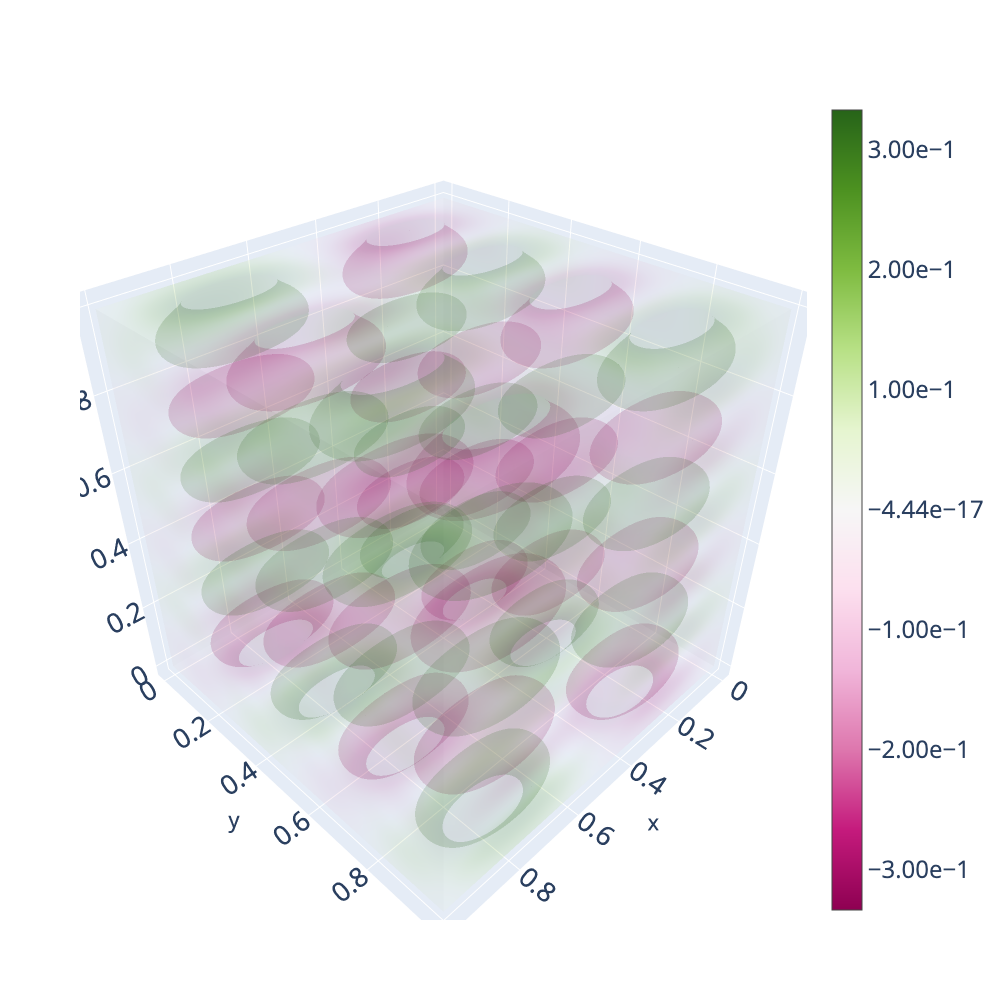
\includegraphics[width=\linewidth]{pictures/1_L1_128_analytical.png}
  \caption{$u_{analytical}$}
\end{subfigure}%
\begin{subfigure}{.33\textwidth}
  \centering
  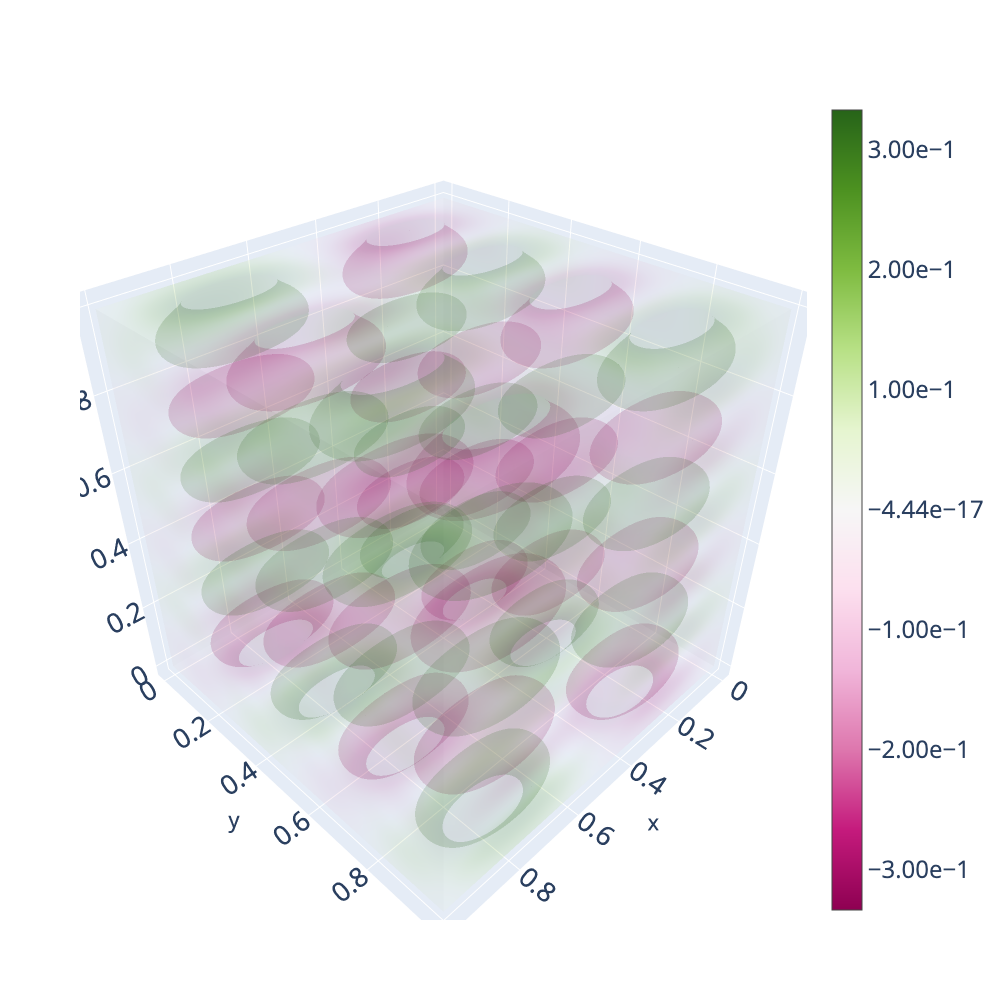
\includegraphics[width=\linewidth]{pictures/1_L1_128_calculated.png}
  \caption{$u_{calculated}$}
\end{subfigure}%
\begin{subfigure}{.33\textwidth}
  \centering
  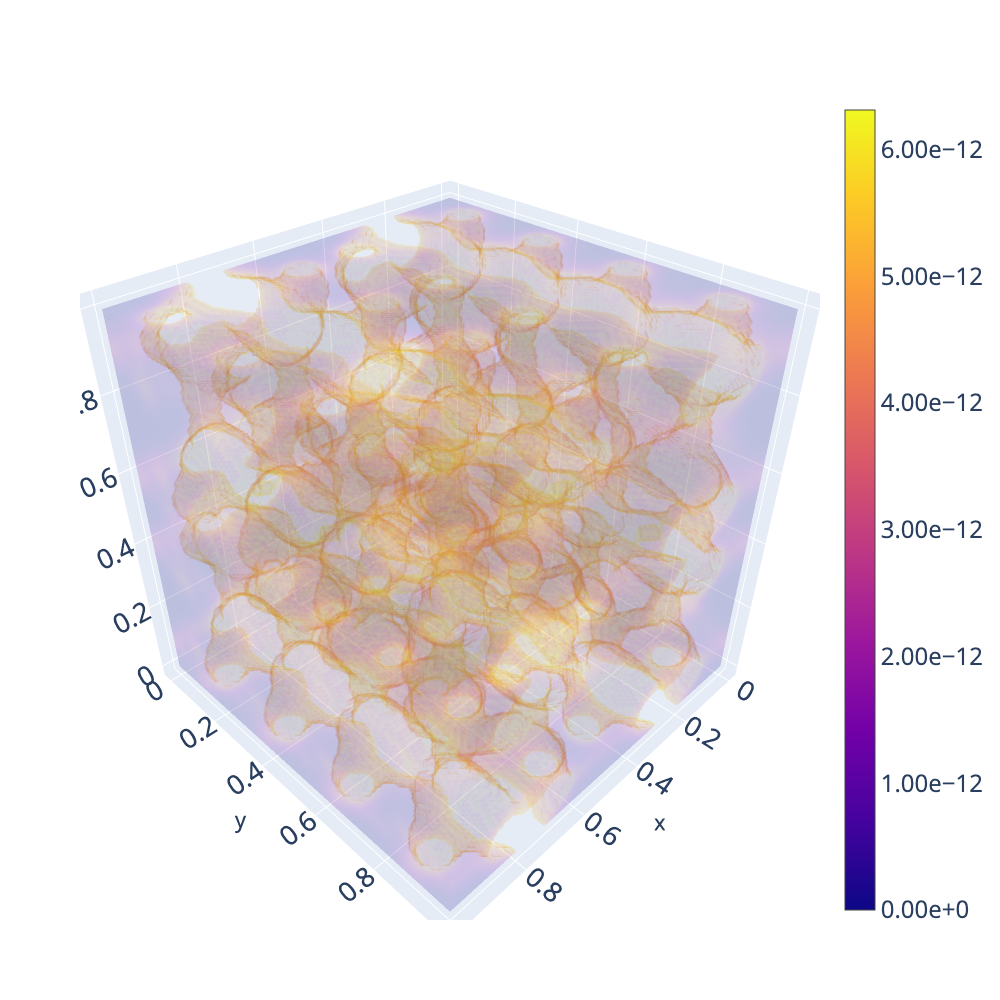
\includegraphics[width=\linewidth]{pictures/1_L1_128_diff.png}
  \caption{погрешность}
\end{subfigure}%
\caption{1 эпоха}
\label{fig:fig}
\end{figure}

\begin{figure}[H]
\begin{subfigure}{.33\textwidth}
  \centering
  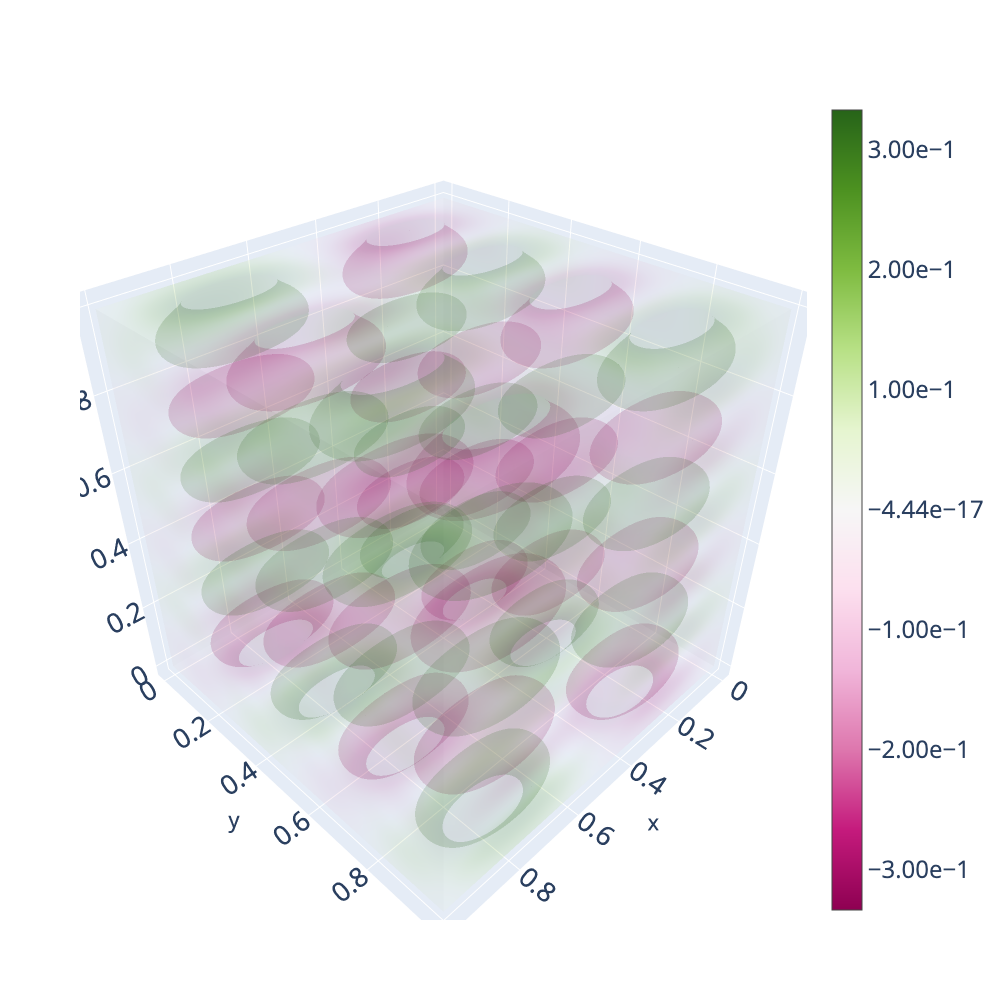
\includegraphics[width=\linewidth]{pictures/10_L1_128_analytical.png}
  \caption{$u_{analytical}$}
\end{subfigure}%
\begin{subfigure}{.33\textwidth}
  \centering
  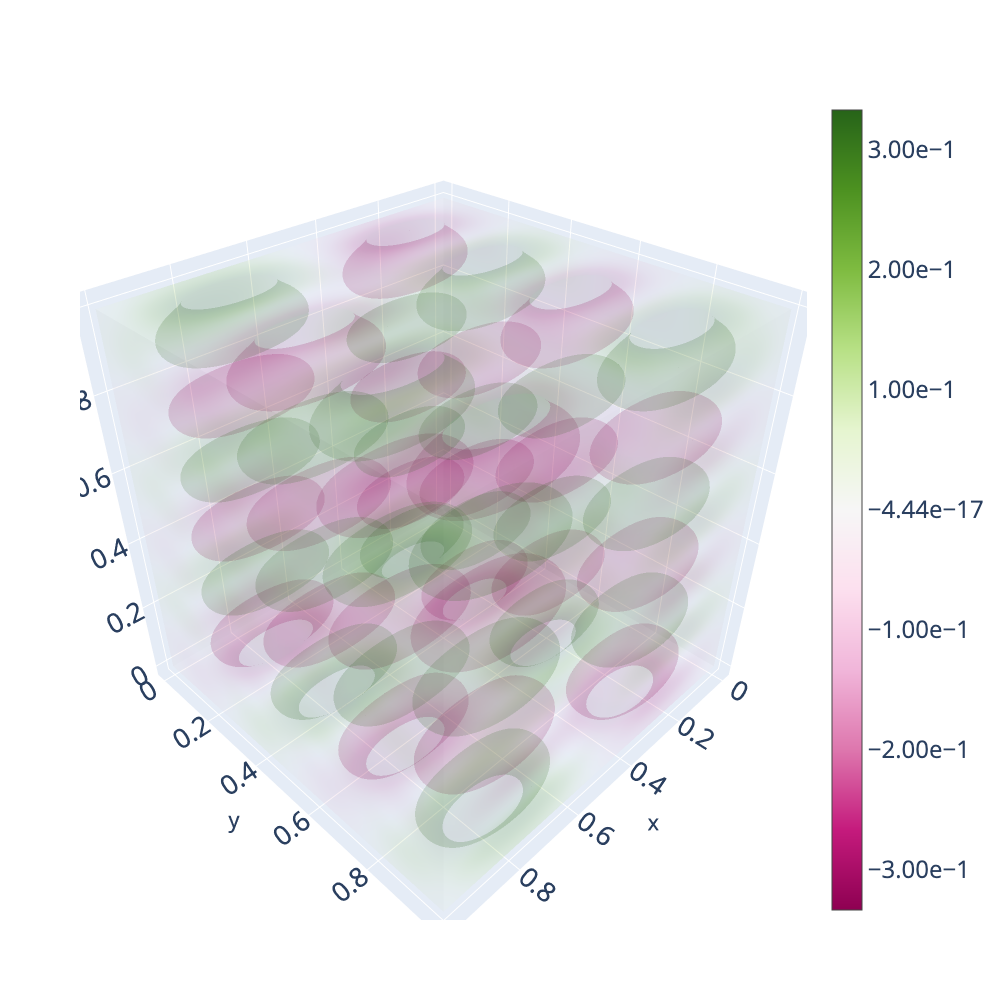
\includegraphics[width=\linewidth]{pictures/10_L1_128_calculated.png}
  \caption{$u_{calculated}$}
\end{subfigure}%
\begin{subfigure}{.33\textwidth}
  \centering
  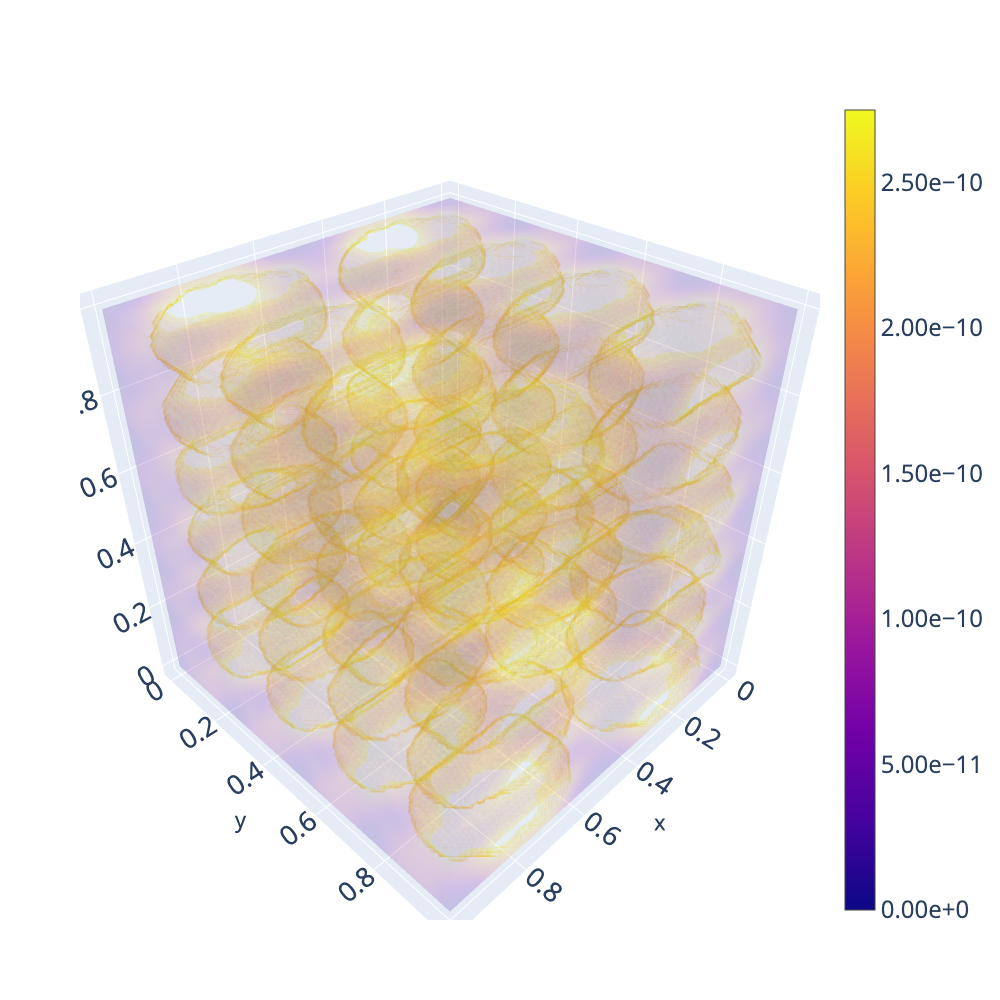
\includegraphics[width=\linewidth]{pictures/10_L1_128_diff.png}
  \caption{погрешность}
\end{subfigure}%
\caption{10 эпоха}
\label{fig:fig}
\end{figure}

\begin{figure}[H]
\begin{subfigure}{.33\textwidth}
  \centering
  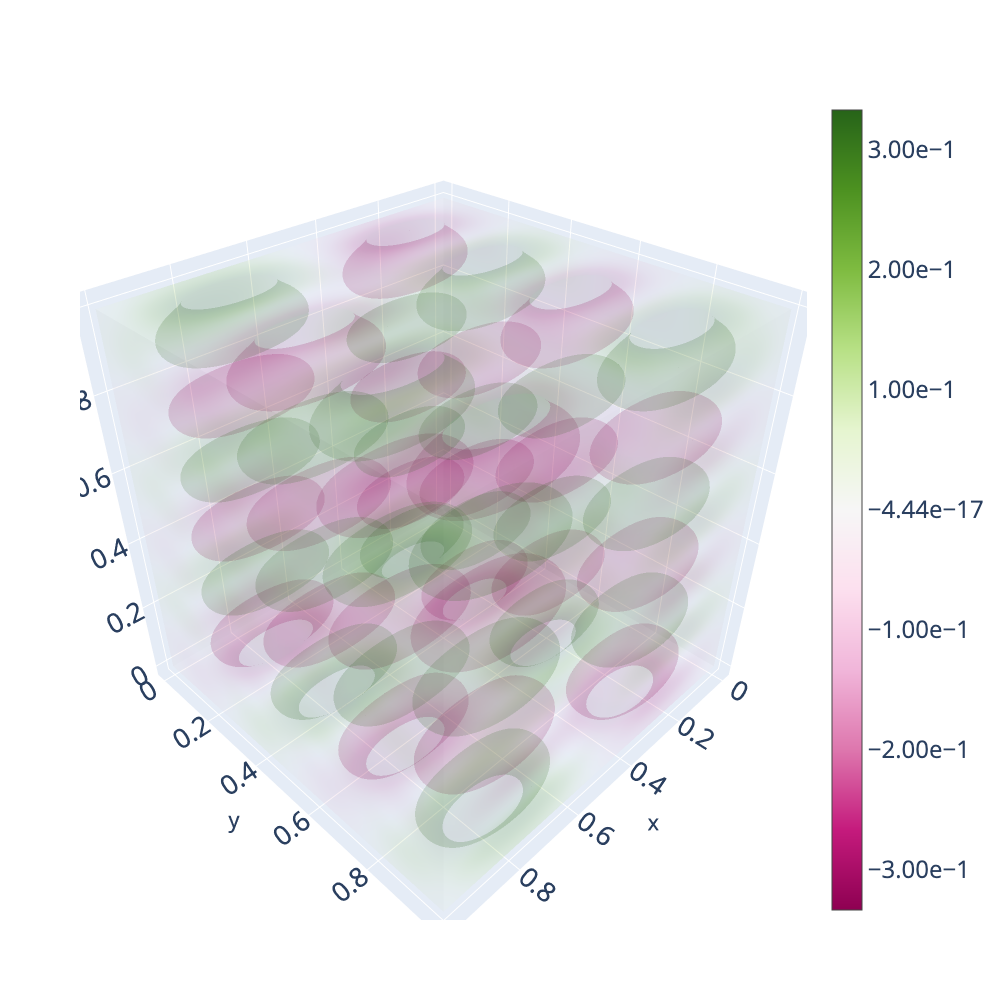
\includegraphics[width=\linewidth]{pictures/19_L1_128_analytical.png}
  \caption{$u_{analytical}$}
\end{subfigure}%
\begin{subfigure}{.33\textwidth}
  \centering
  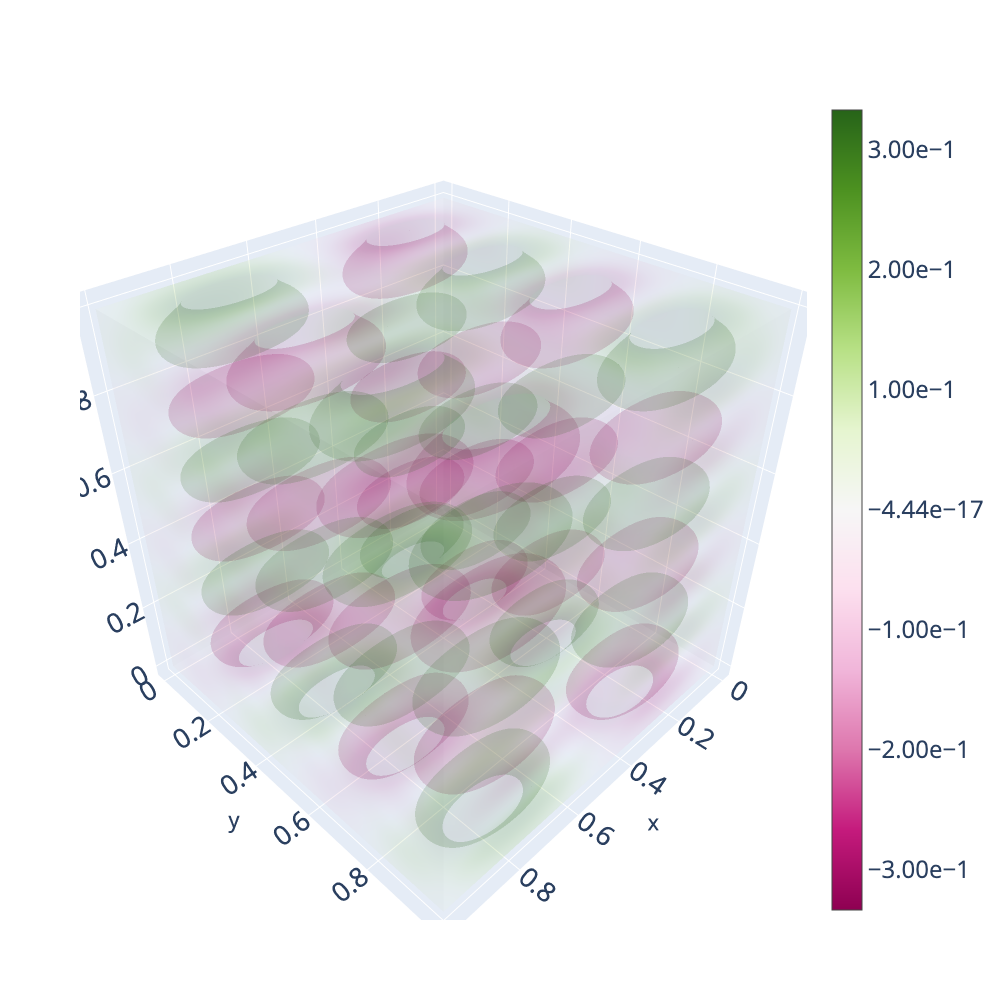
\includegraphics[width=\linewidth]{pictures/19_L1_128_calculated.png}
  \caption{$u_{calculated}$}
\end{subfigure}%
\begin{subfigure}{.33\textwidth}
  \centering
  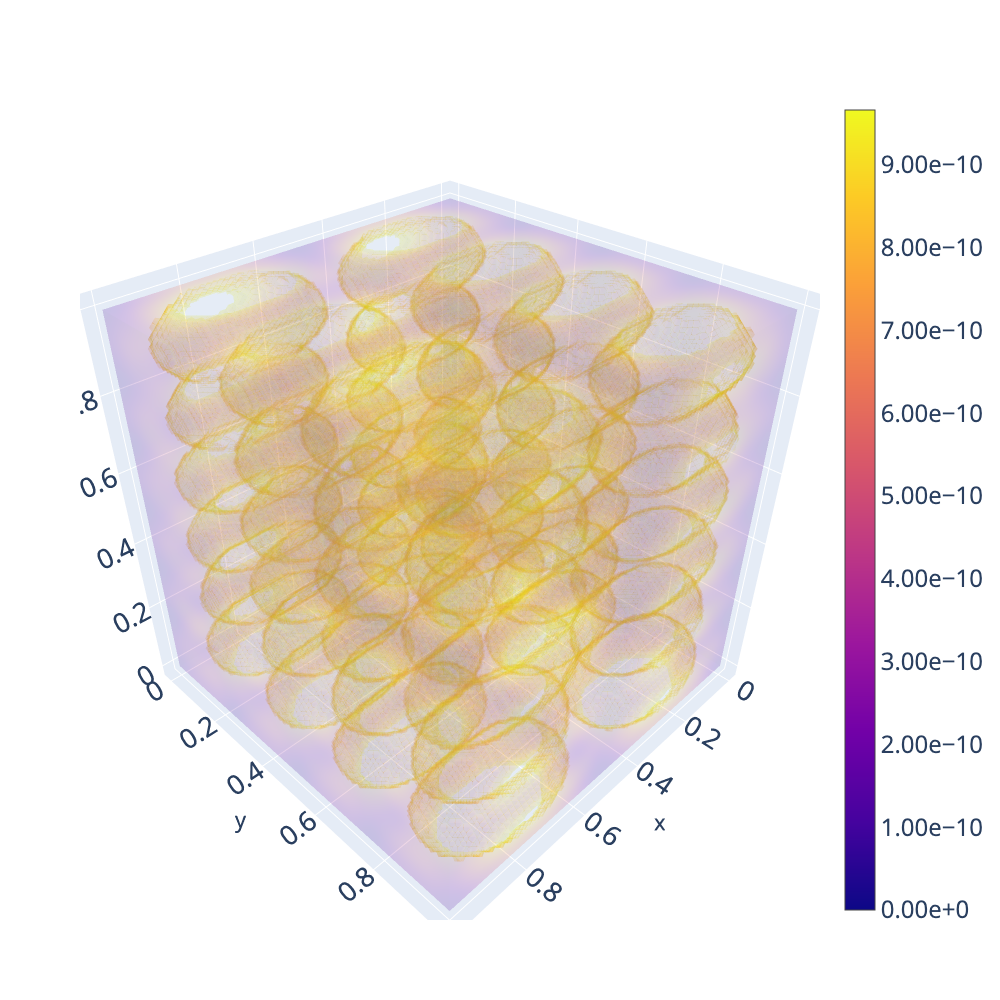
\includegraphics[width=\linewidth]{pictures/19_L1_128_diff.png}
  \caption{погрешность}
\end{subfigure}%
\caption{20 эпоха}
\label{fig:fig}
\end{figure}

\begin{figure}[H]
\begin{subfigure}{.5\textwidth}
  \centering
  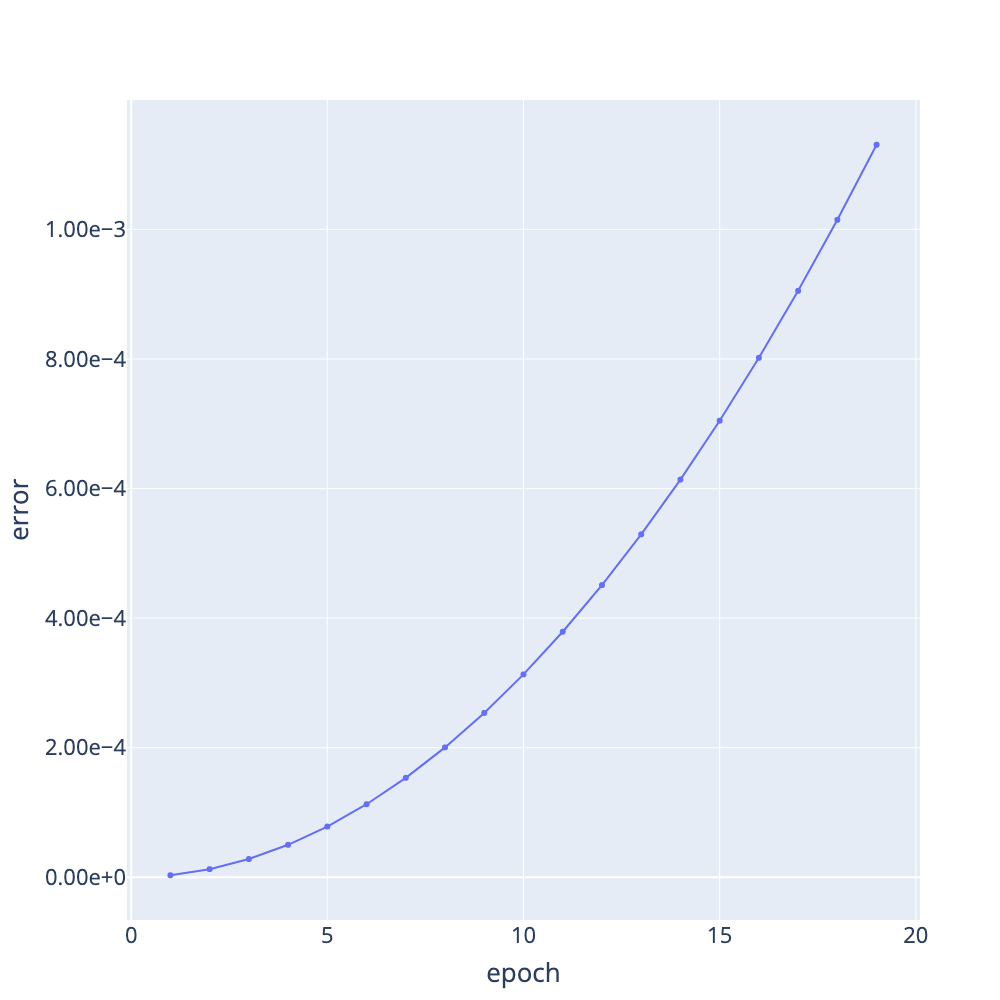
\includegraphics[width=\linewidth]{pictures/L1_128_errs.png}
  \caption{Погрешность от эпохи}
\end{subfigure}%
\begin{subfigure}{.5\textwidth}
  \centering
  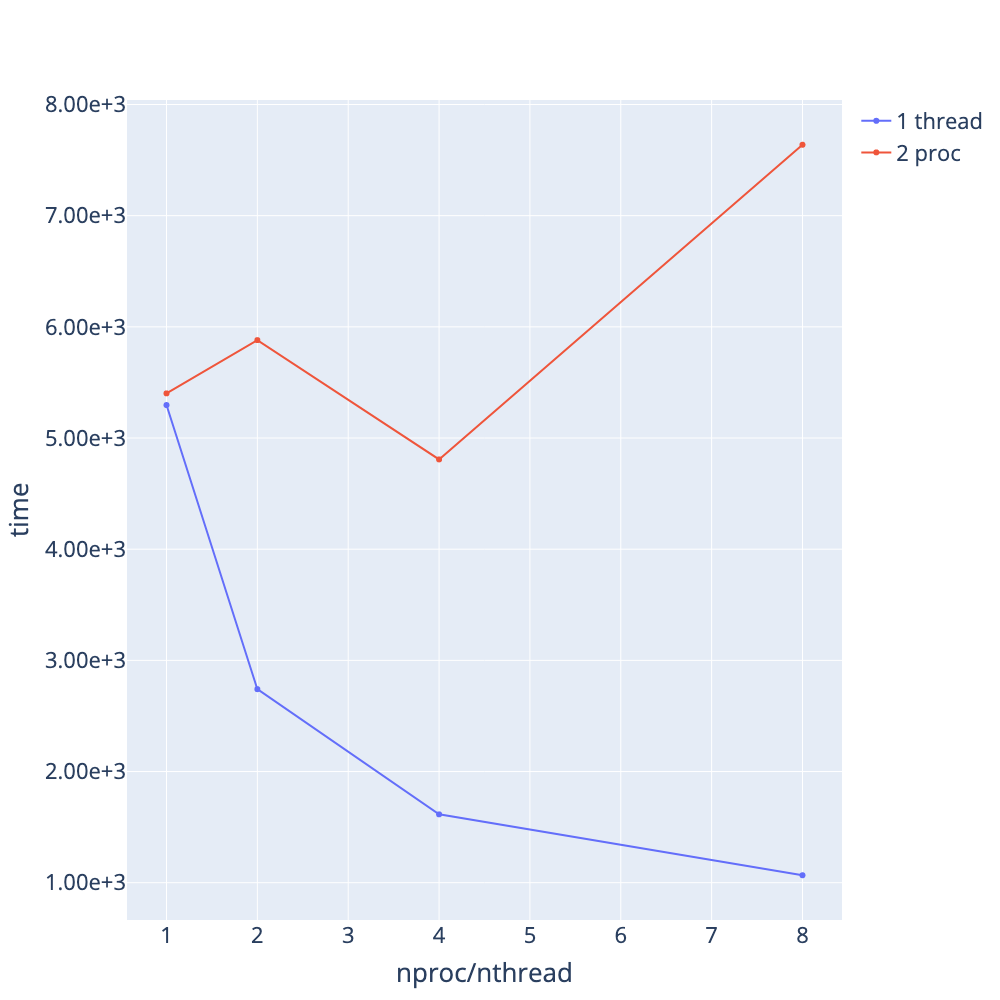
\includegraphics[width=\linewidth]{pictures/L1_128_perf.png}
  \caption{Время работы от конфигурации}
\end{subfigure}%
\end{figure}


\subsubsection{Графики для N=256}

\begin{figure}[H]
\begin{subfigure}{.33\textwidth}
  \centering
  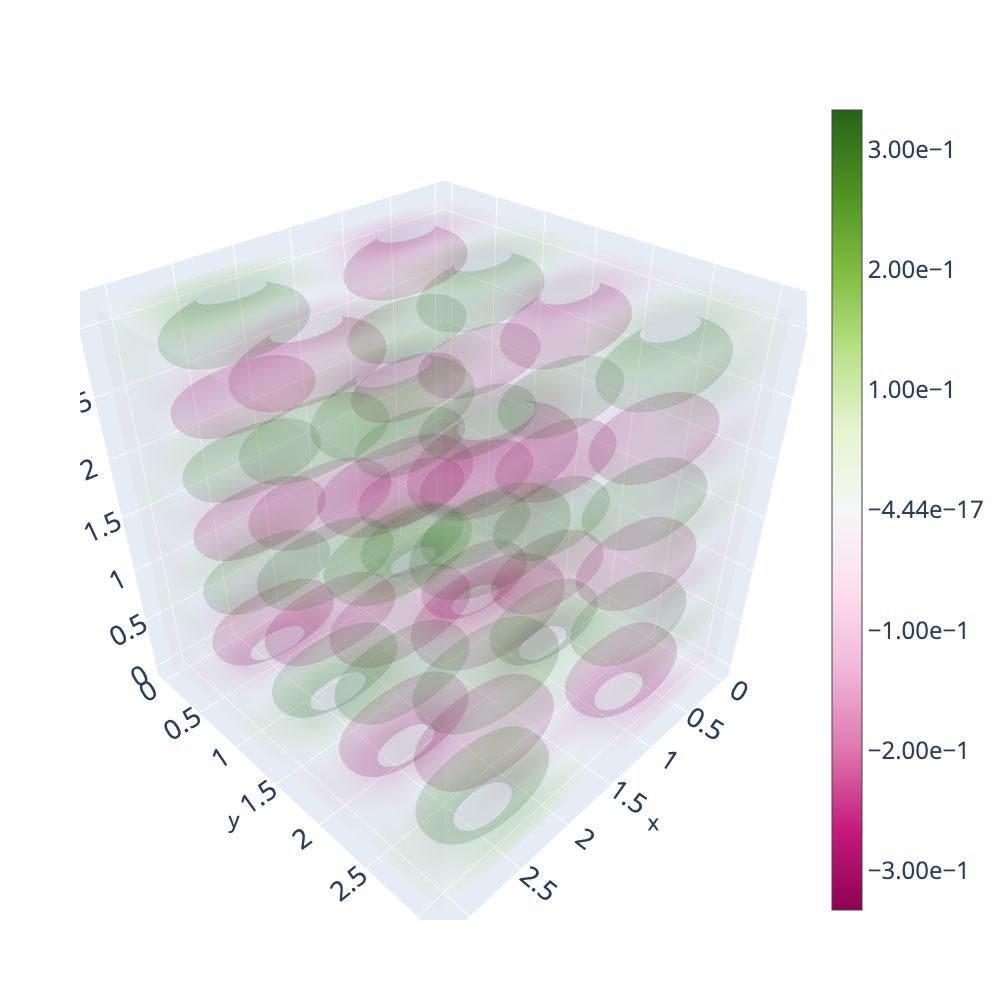
\includegraphics[width=\linewidth]{pictures/1_L1_256_analytical.png}
  \caption{$u_{analytical}$}
\end{subfigure}%
\begin{subfigure}{.33\textwidth}
  \centering
  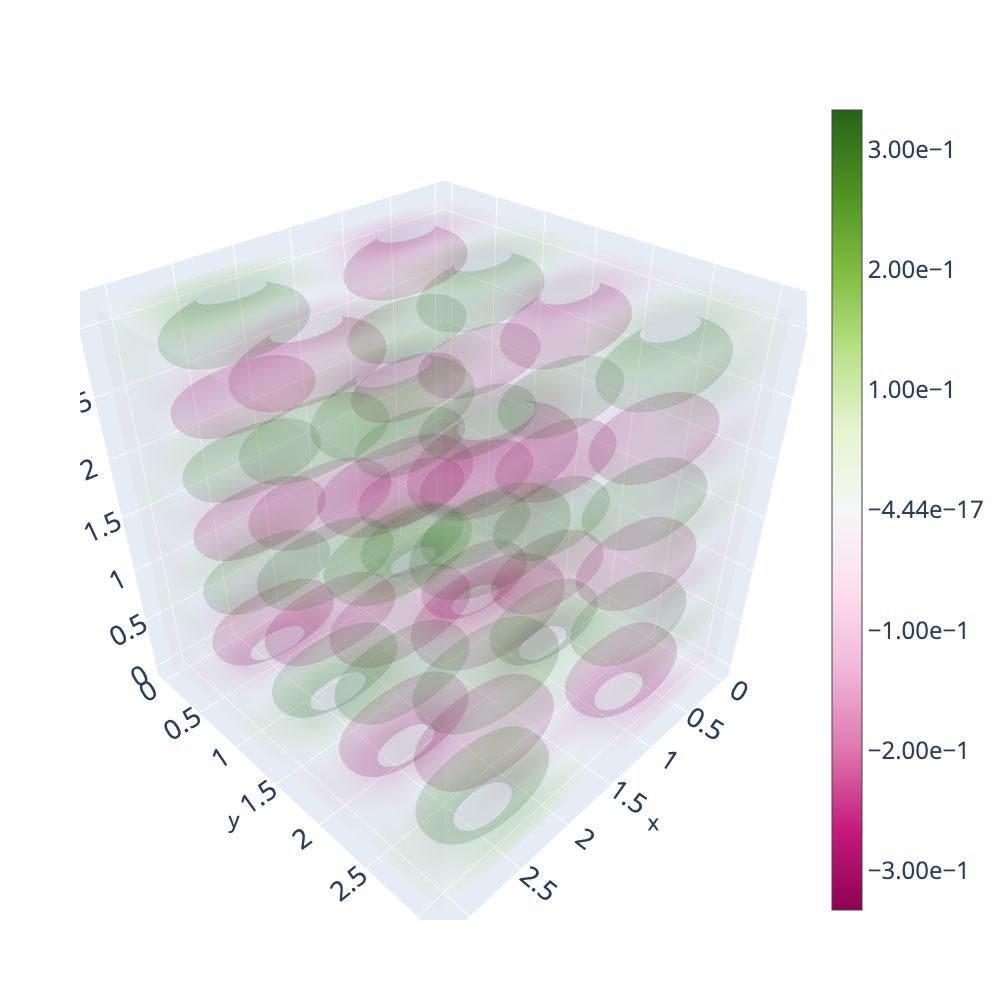
\includegraphics[width=\linewidth]{pictures/1_L1_256_calculated.png}
  \caption{$u_{calculated}$}
\end{subfigure}%
\begin{subfigure}{.33\textwidth}
  \centering
  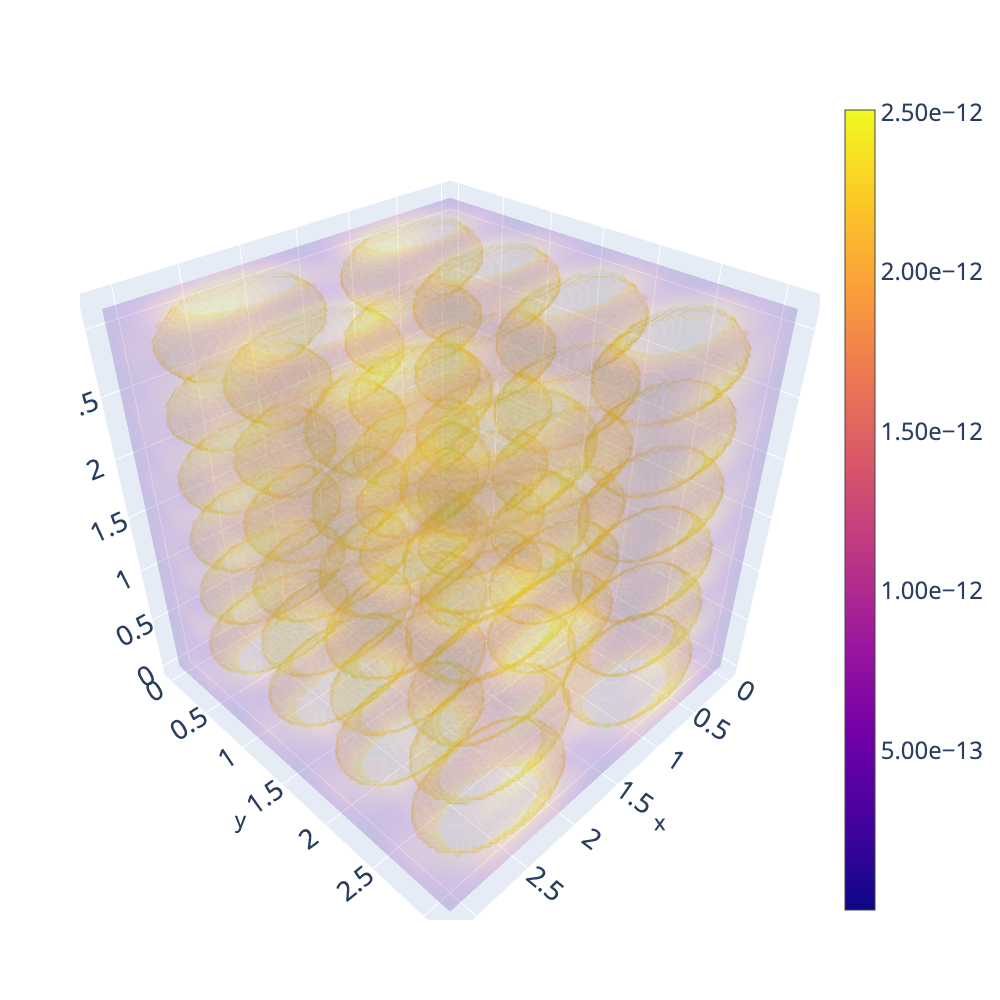
\includegraphics[width=\linewidth]{pictures/1_L1_256_diff.png}
  \caption{погрешность}
\end{subfigure}%
\caption{1 эпоха}
\label{fig:fig}
\end{figure}

\begin{figure}[H]
\begin{subfigure}{.33\textwidth}
  \centering
  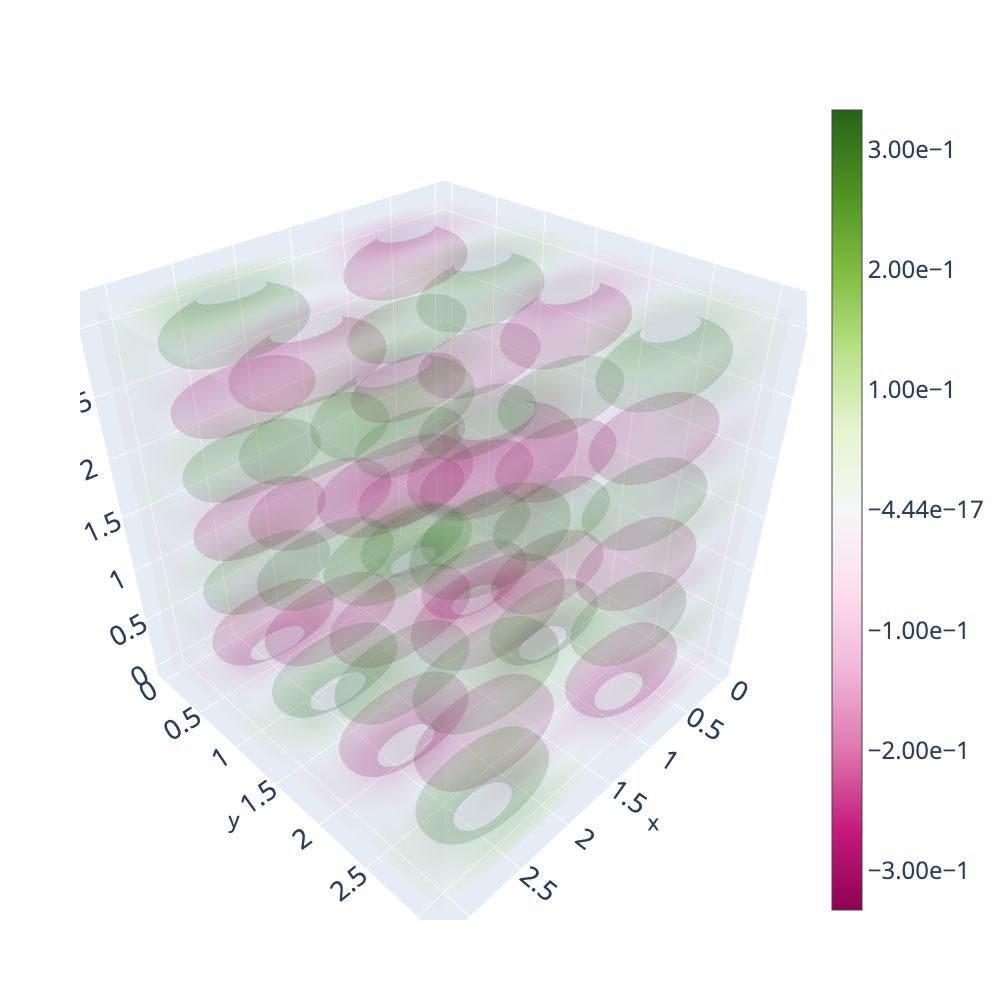
\includegraphics[width=\linewidth]{pictures/10_L1_256_analytical.png}
  \caption{$u_{analytical}$}
\end{subfigure}%
\begin{subfigure}{.33\textwidth}
  \centering
  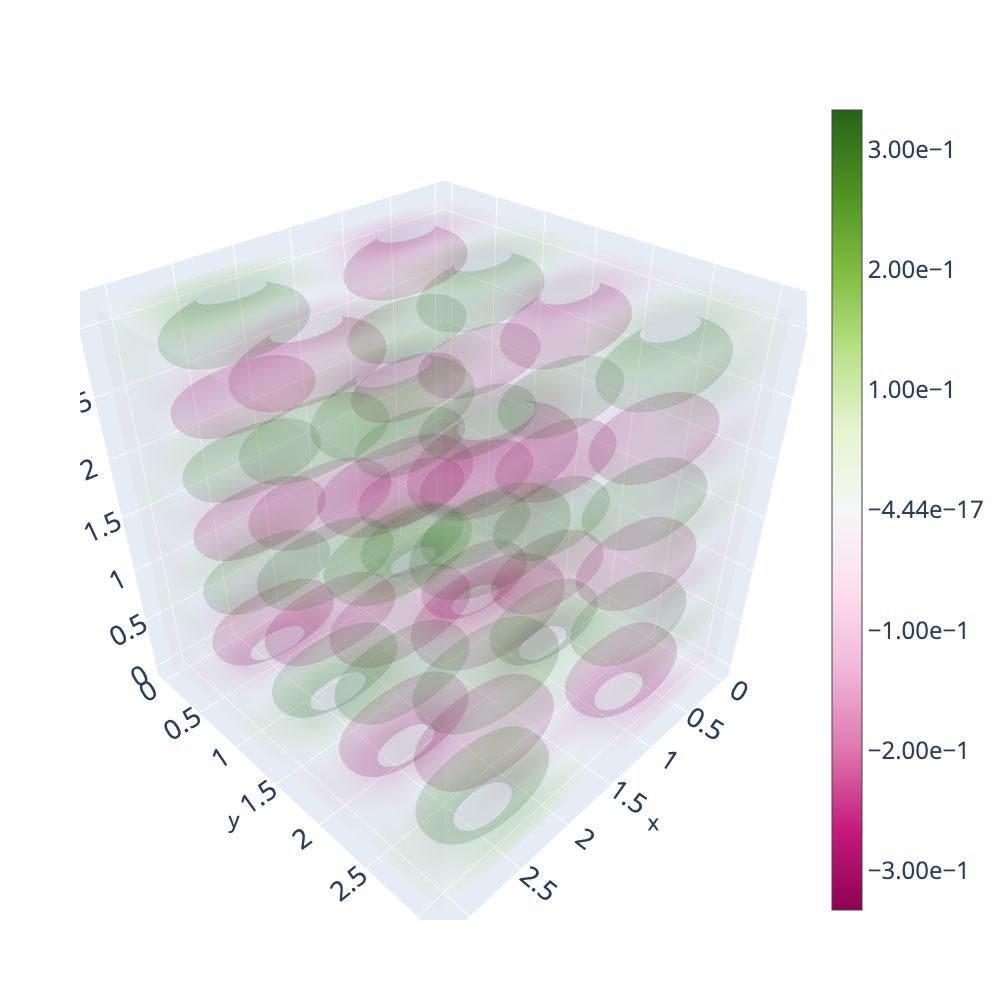
\includegraphics[width=\linewidth]{pictures/10_L1_256_calculated.png}
  \caption{$u_{calculated}$}
\end{subfigure}%
\begin{subfigure}{.33\textwidth}
  \centering
  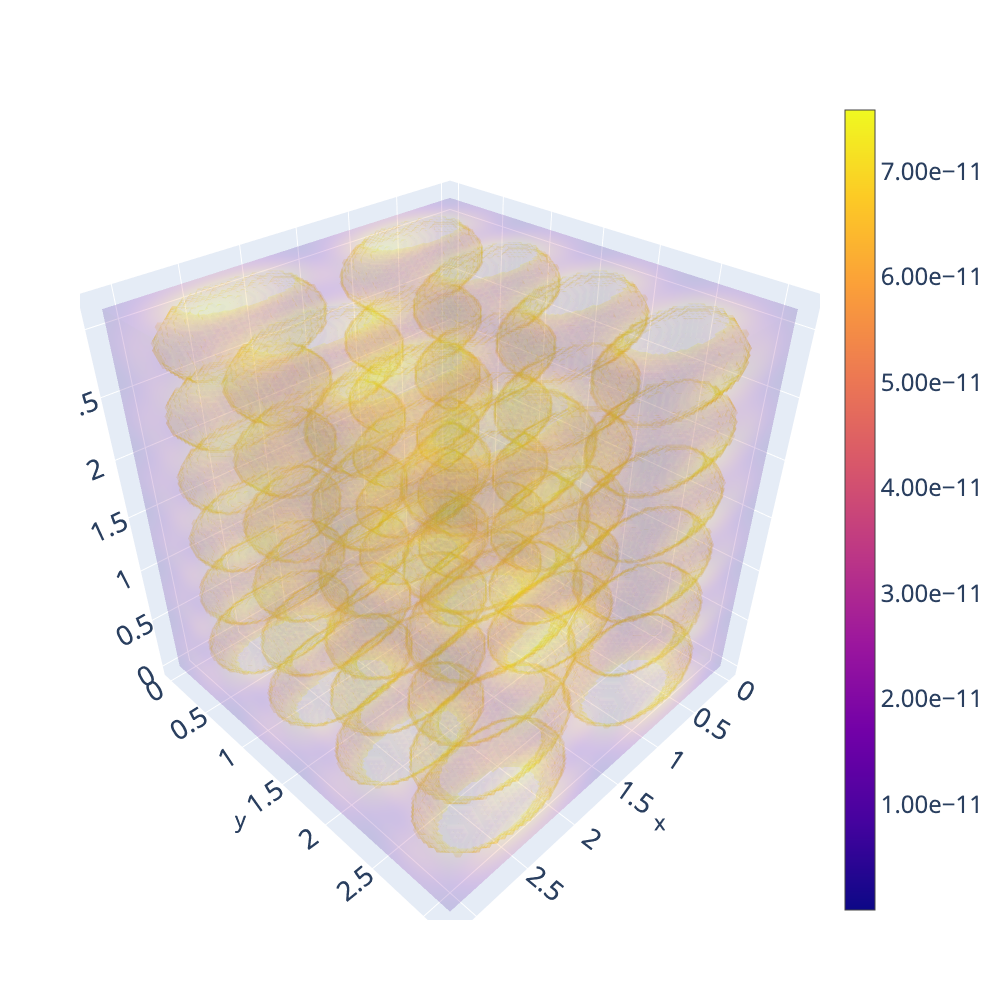
\includegraphics[width=\linewidth]{pictures/10_L1_256_diff.png}
  \caption{погрешность}
\end{subfigure}%
\caption{10 эпоха}
\label{fig:fig}
\end{figure}

\begin{figure}[H]
\begin{subfigure}{.33\textwidth}
  \centering
  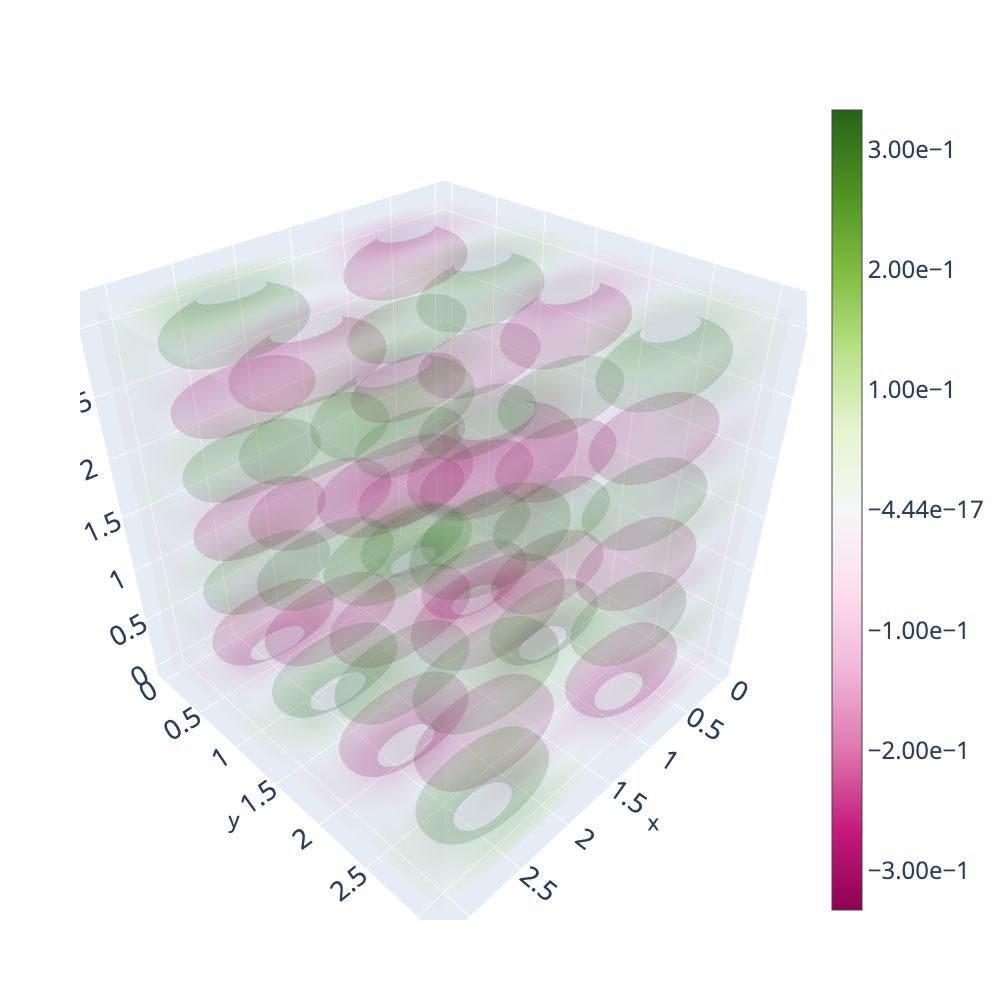
\includegraphics[width=\linewidth]{pictures/19_L1_256_analytical.png}
  \caption{$u_{analytical}$}
\end{subfigure}%
\begin{subfigure}{.33\textwidth}
  \centering
  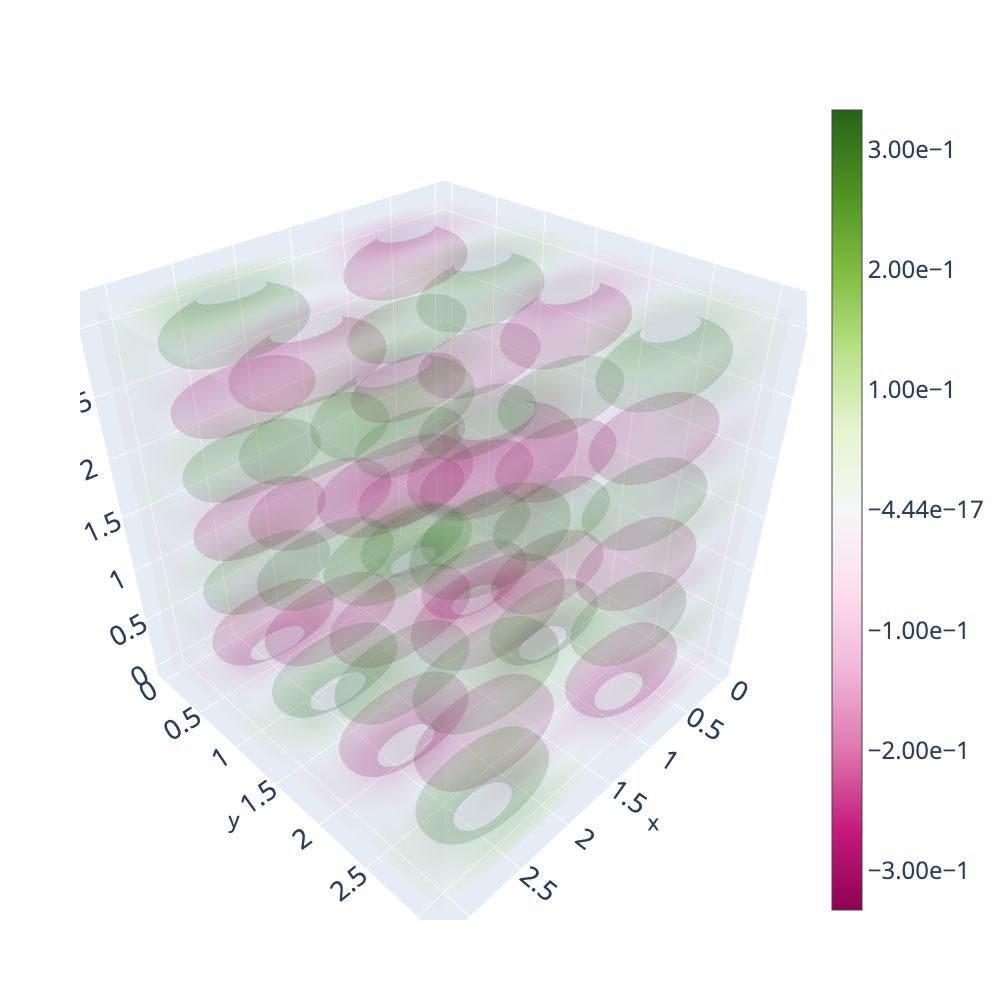
\includegraphics[width=\linewidth]{pictures/19_L1_256_calculated.png}
  \caption{$u_{calculated}$}
\end{subfigure}%
\begin{subfigure}{.33\textwidth}
  \centering
  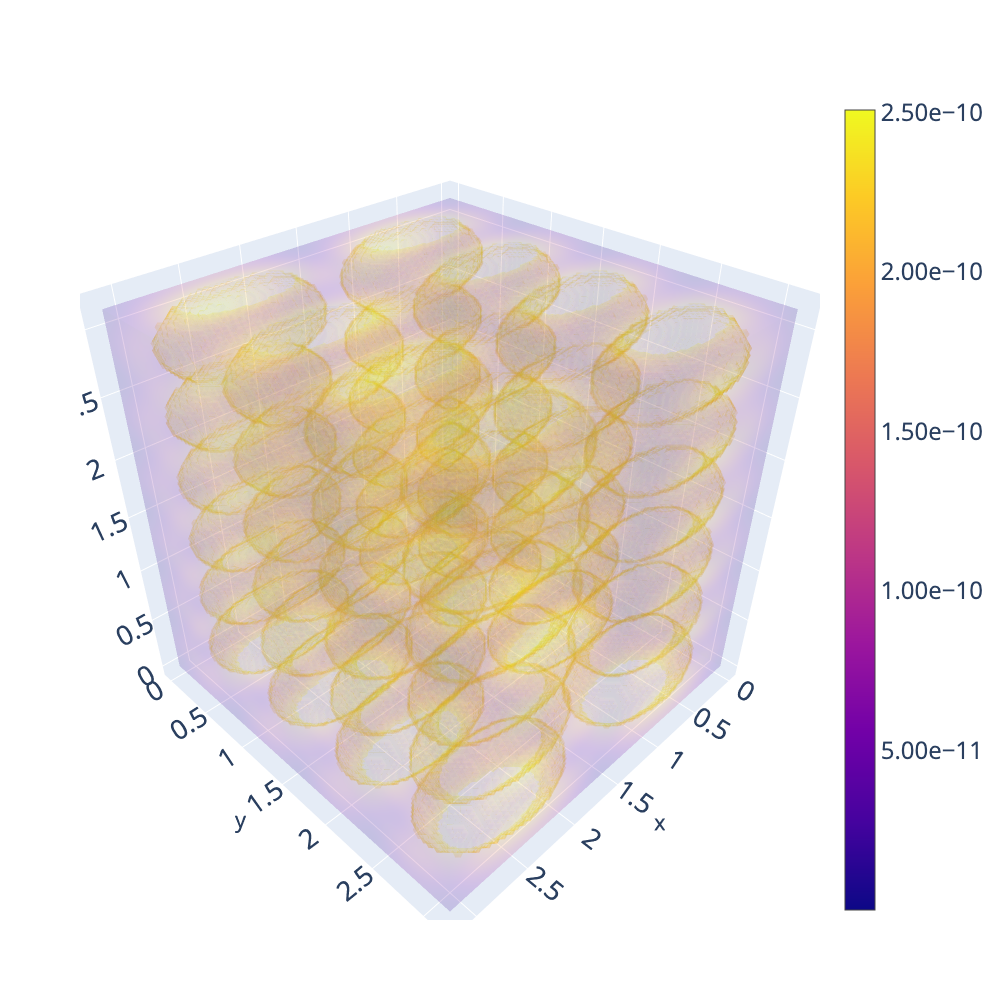
\includegraphics[width=\linewidth]{pictures/19_L1_256_diff.png}
  \caption{погрешность}
\end{subfigure}%
\caption{20 эпоха}
\label{fig:fig}
\end{figure}

\begin{figure}[H]
\begin{subfigure}{.5\textwidth}
  \centering
  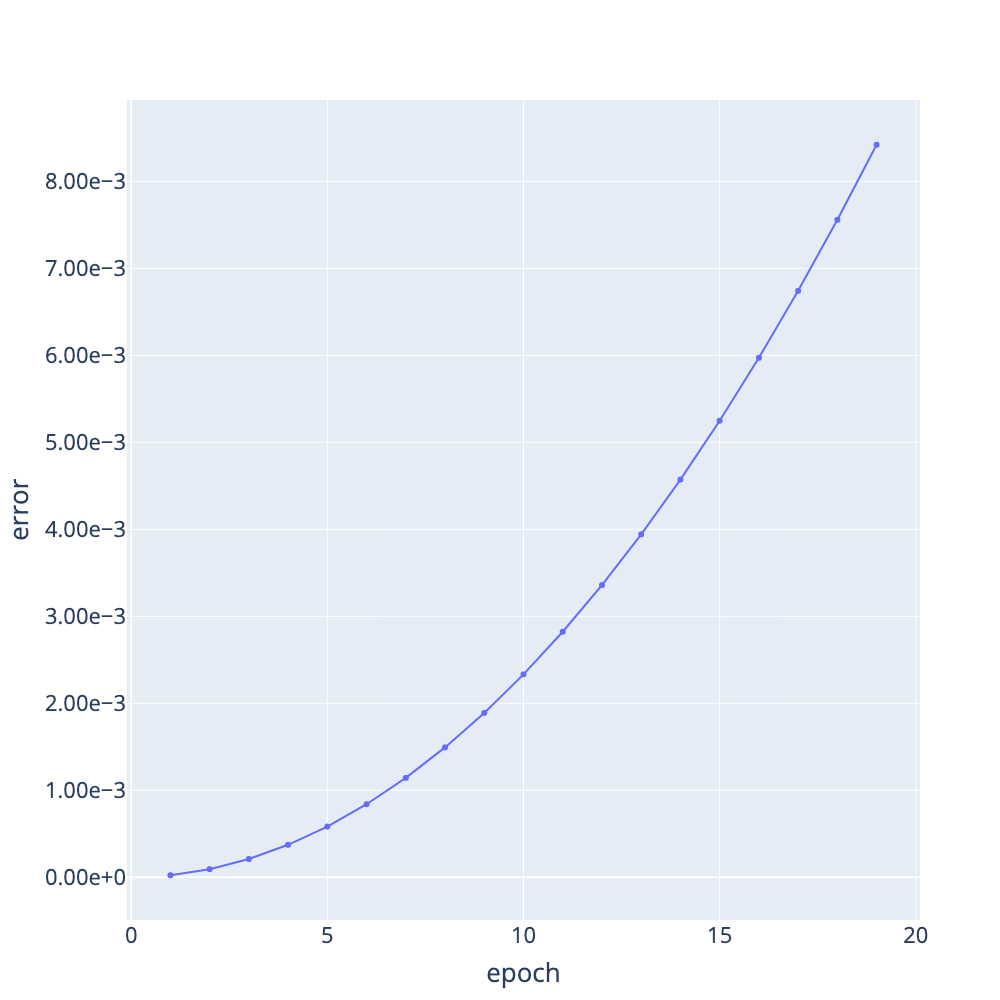
\includegraphics[width=\linewidth]{pictures/L1_256_errs.png}
  \caption{Погрешность от эпохи}
\end{subfigure}%
\begin{subfigure}{.5\textwidth}
  \centering
  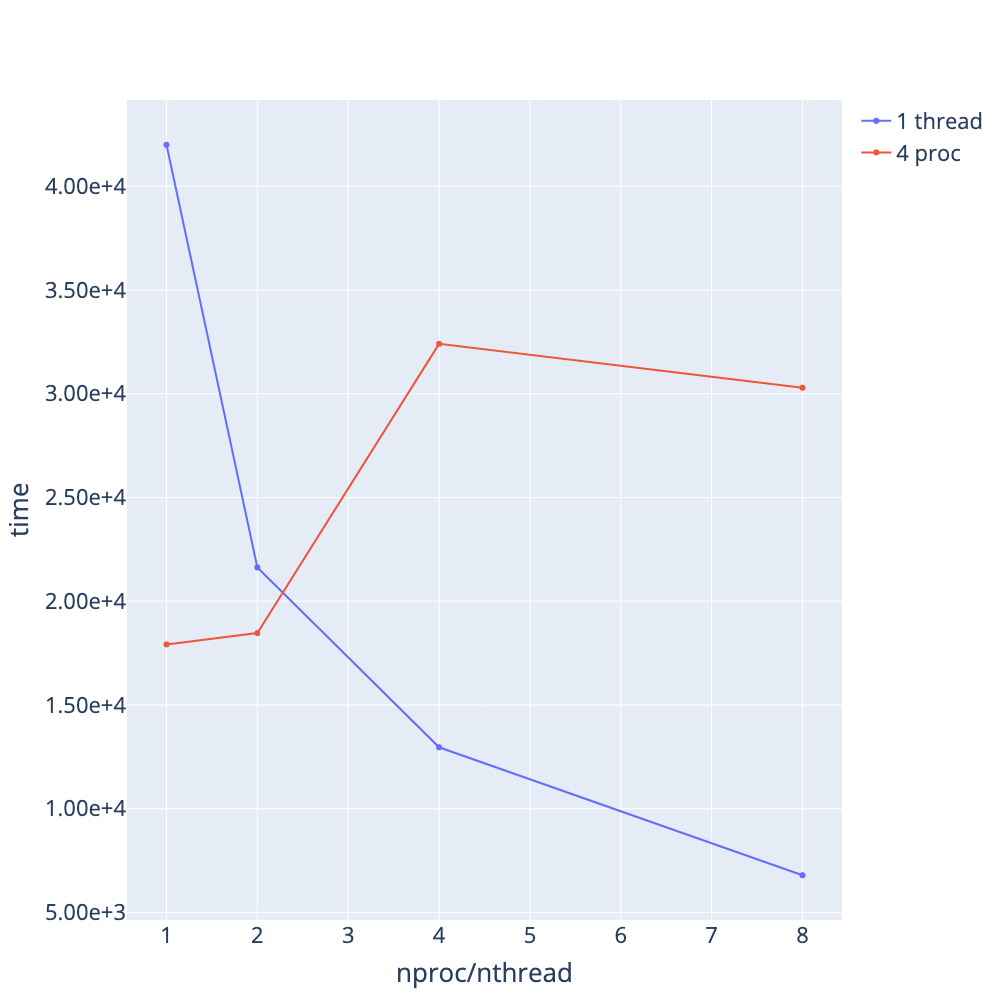
\includegraphics[width=\linewidth]{pictures/L1_256_perf.png}
  \caption{Время работы от конфигурации}
\end{subfigure}%
\end{figure}

\newpage
\subsection{L = $\pi$}

{
\centering
\noindent\begin{tabular}{|p{2cm}|p{2cm}|p{2.5cm}|p{2.5cm}|p{2cm}|p{2.5cm}|}
    \hline
    \textit{Число MPI процессов }$N_p$ & \textit{Число OpenMP нитей} & \textit{Число точек сетки }$N^3$ & \textit{Время решения T (ms)} & \textit{Ускорение S} & \textit{Погрешность }$\delta$ \\
    \hline
    1 & 1 & $128^3$ & 5743.76 & 1 & 0.000126933 \\
    2 & 1 & $128^3$ & 3214.88 & 1.79 & 0.000126933 \\
    4 & 1 & $128^3$ & 2137.36 & 2.69 & 0.000126933 \\
    8 & 1 & $128^3$ & 1089.79 & 5.27 & 0.000126933 \\
    \hline
    2 & 1 & $128^3$ & 7928.95 & 1 & 0.000126933 \\
    2 & 2 & $128^3$ & 9870.61 & 0.8 & 0.000126933 \\
    2 & 4 & $128^3$ & 12763.1 & 0.62 & 0.000126933 \\
    2 & 8 & $128^3$ & 17839 & 0.44 & 0.000126933 \\
    \hline
    \hline
    1 & 1 & $256^3$ & 45737.6 & 1 & 0.00094537 \\
    2 & 1 & $256^3$ & 28286.4 & 1.62 & 0.00094537 \\
    4 & 1 & $256^3$ & 13910.3 & 3.29 & 0.00094537 \\
    8 & 1 & $256^3$ & 9115.46 & 5.02 & 0.00094537 \\
    \hline
    4 & 1 & $256^3$ & 19964.4 & 1 & 0.00094537 \\
    4 & 2 & $256^3$ & 20680.2 & 0.97 & 0.00094537 \\
    4 & 4 & $256^3$ & 24246.2 & 0.82 & 0.00094537 \\
    4 & 8 & $256^3$ & 30478.3 & 0.66 & 0.00094537 \\
    \hline
    
\end{tabular}
}

\subsubsection{Графики для N=128}

\begin{figure}[H]
\begin{subfigure}{.33\textwidth}
  \centering
  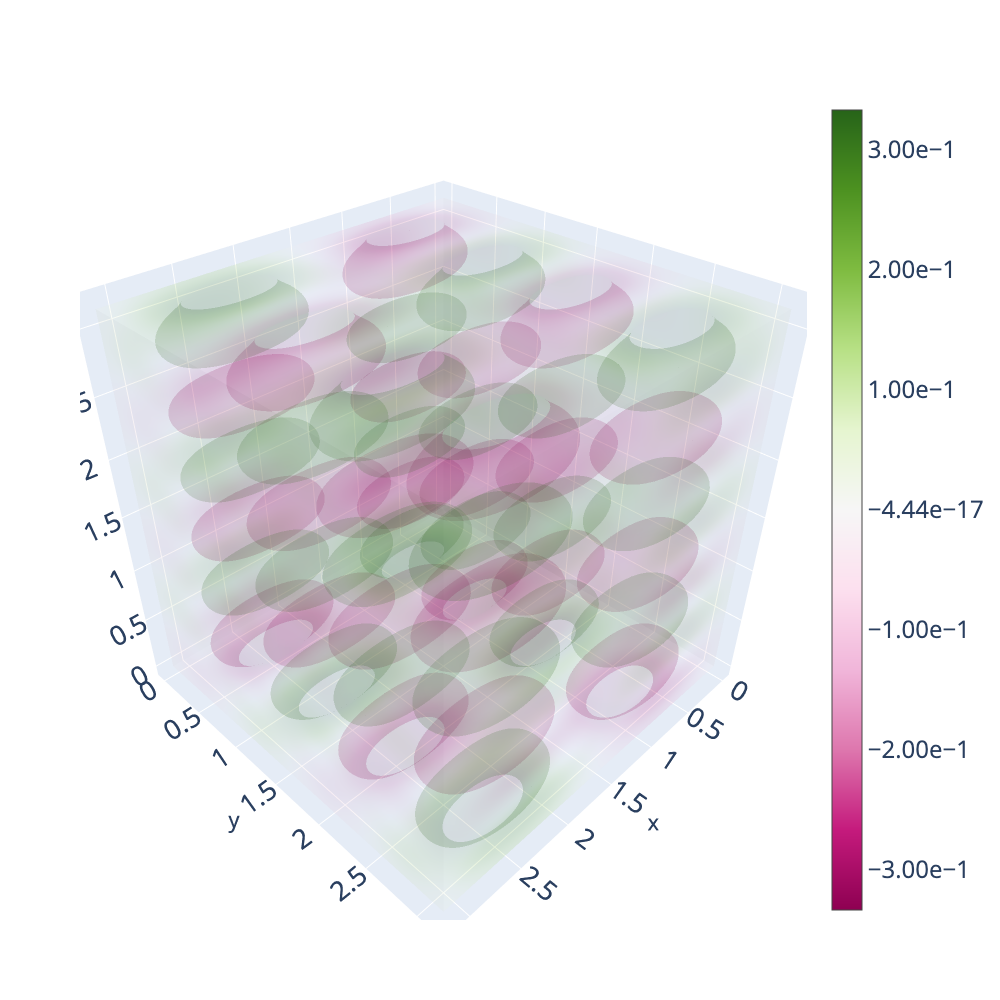
\includegraphics[width=\linewidth]{pictures/1_Lpi_128_analytical.png}
  \caption{$u_{analytical}$}
\end{subfigure}%
\begin{subfigure}{.33\textwidth}
  \centering
  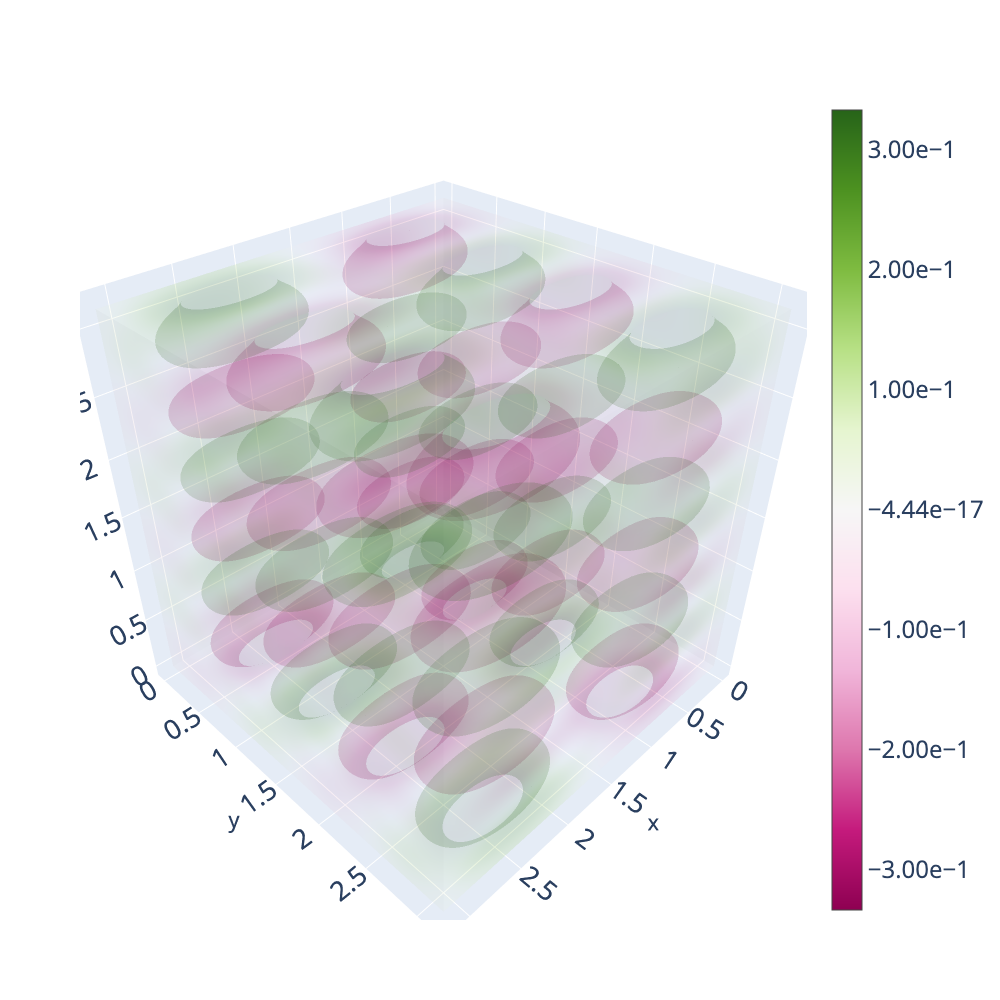
\includegraphics[width=\linewidth]{pictures/1_Lpi_128_calculated.png}
  \caption{$u_{calculated}$}
\end{subfigure}%
\begin{subfigure}{.33\textwidth}
  \centering
  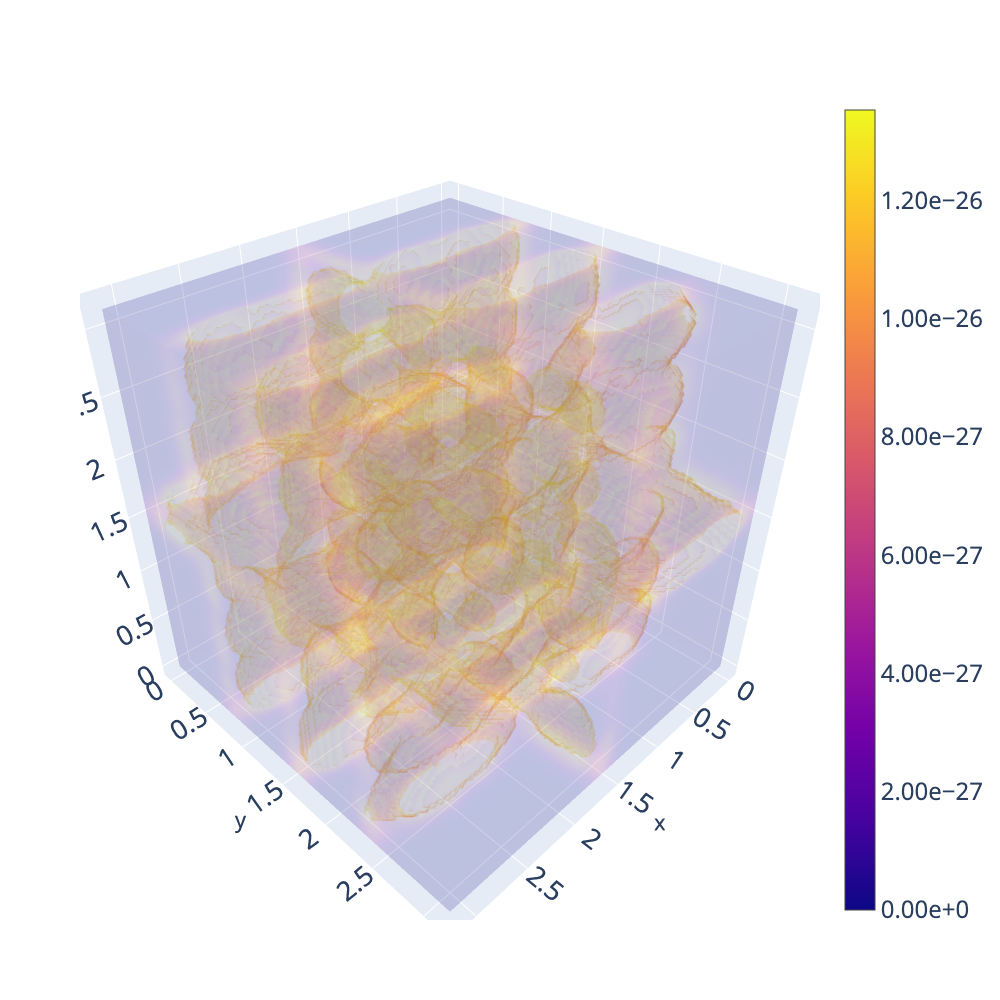
\includegraphics[width=\linewidth]{pictures/1_Lpi_128_diff.png}
  \caption{погрешность}
\end{subfigure}%
\caption{1 эпоха}
\label{fig:fig}
\end{figure}

\begin{figure}[H]
\begin{subfigure}{.33\textwidth}
  \centering
  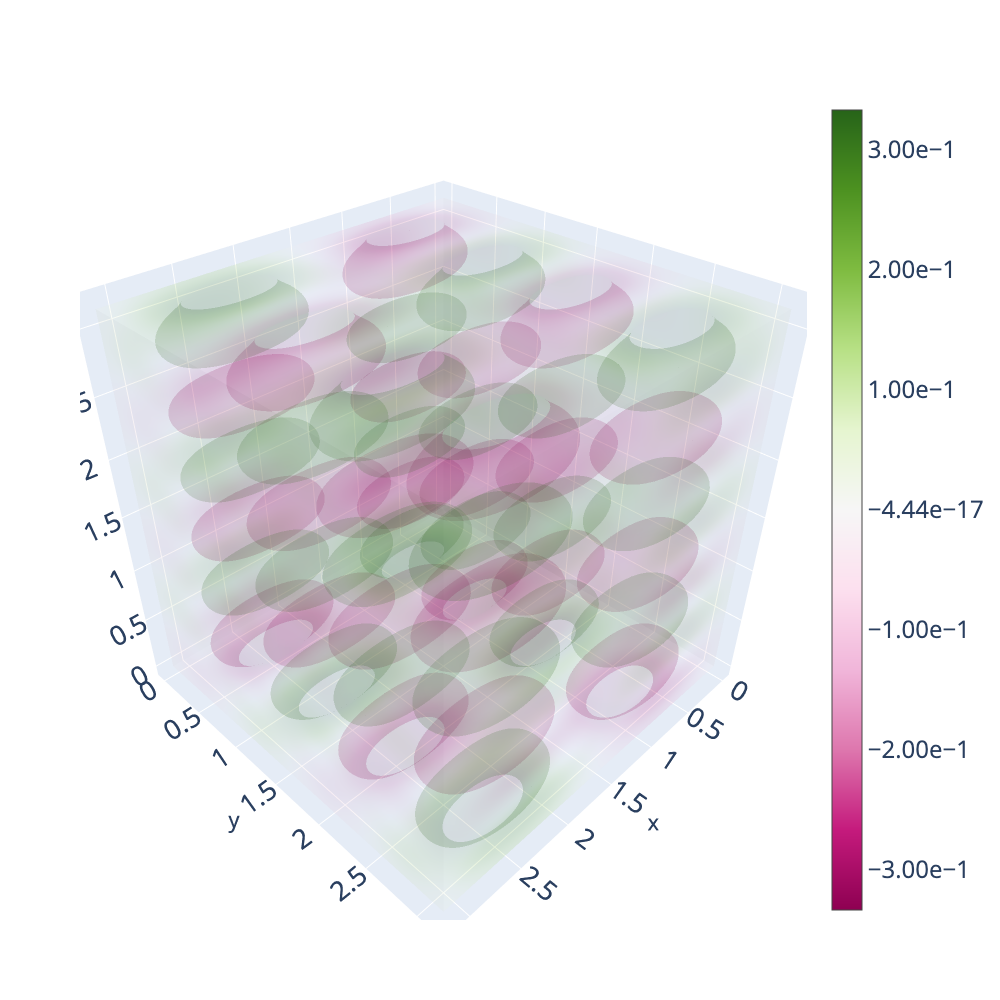
\includegraphics[width=\linewidth]{pictures/10_Lpi_128_analytical.png}
  \caption{$u_{analytical}$}
\end{subfigure}%
\begin{subfigure}{.33\textwidth}
  \centering
  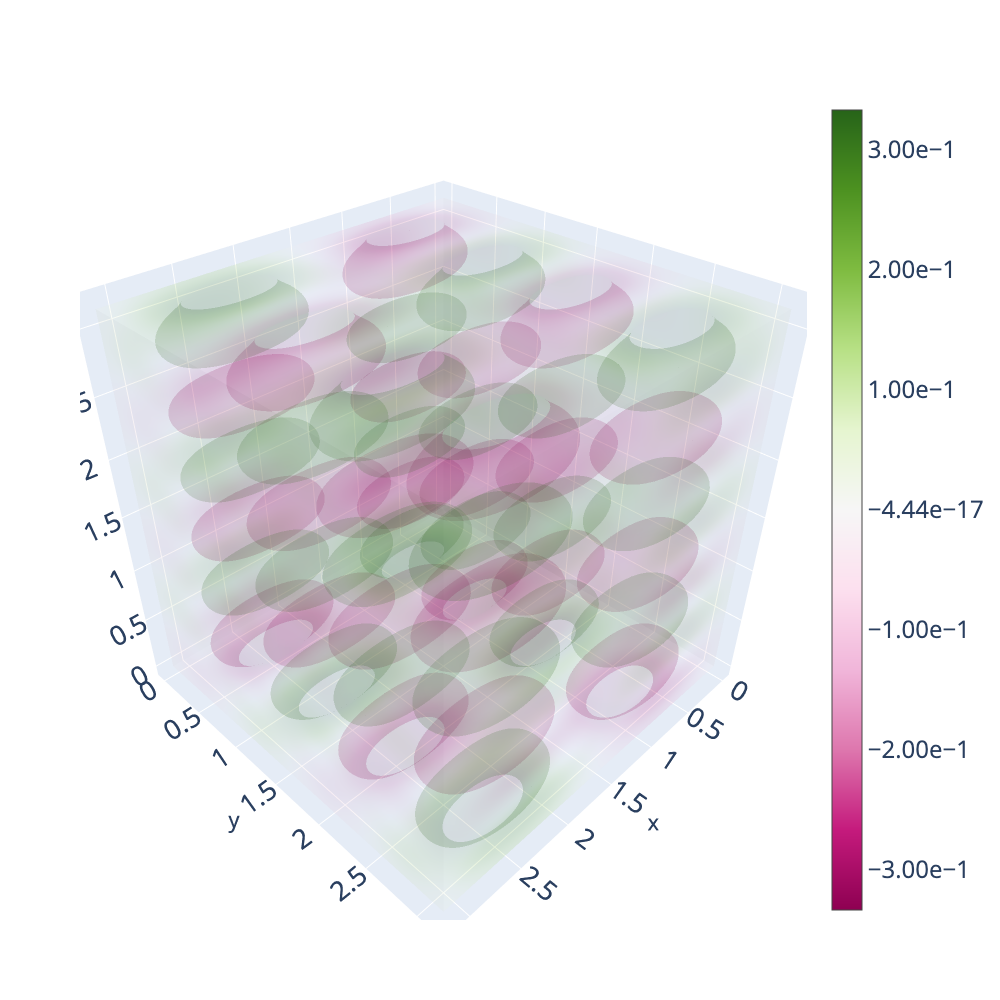
\includegraphics[width=\linewidth]{pictures/10_Lpi_128_calculated.png}
  \caption{$u_{calculated}$}
\end{subfigure}%
\begin{subfigure}{.33\textwidth}
  \centering
  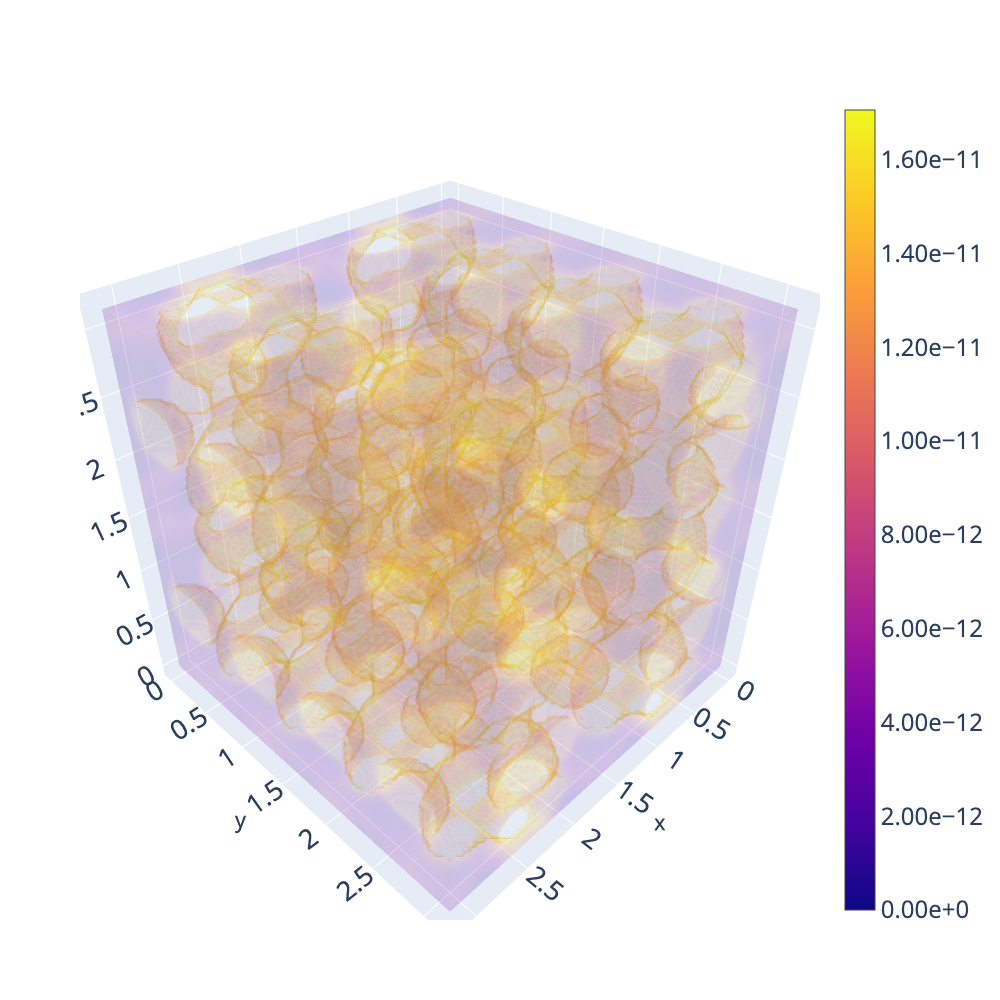
\includegraphics[width=\linewidth]{pictures/10_Lpi_128_diff.png}
  \caption{погрешность}
\end{subfigure}%
\caption{10 эпоха}
\label{fig:fig}
\end{figure}

\begin{figure}[H]
\begin{subfigure}{.33\textwidth}
  \centering
  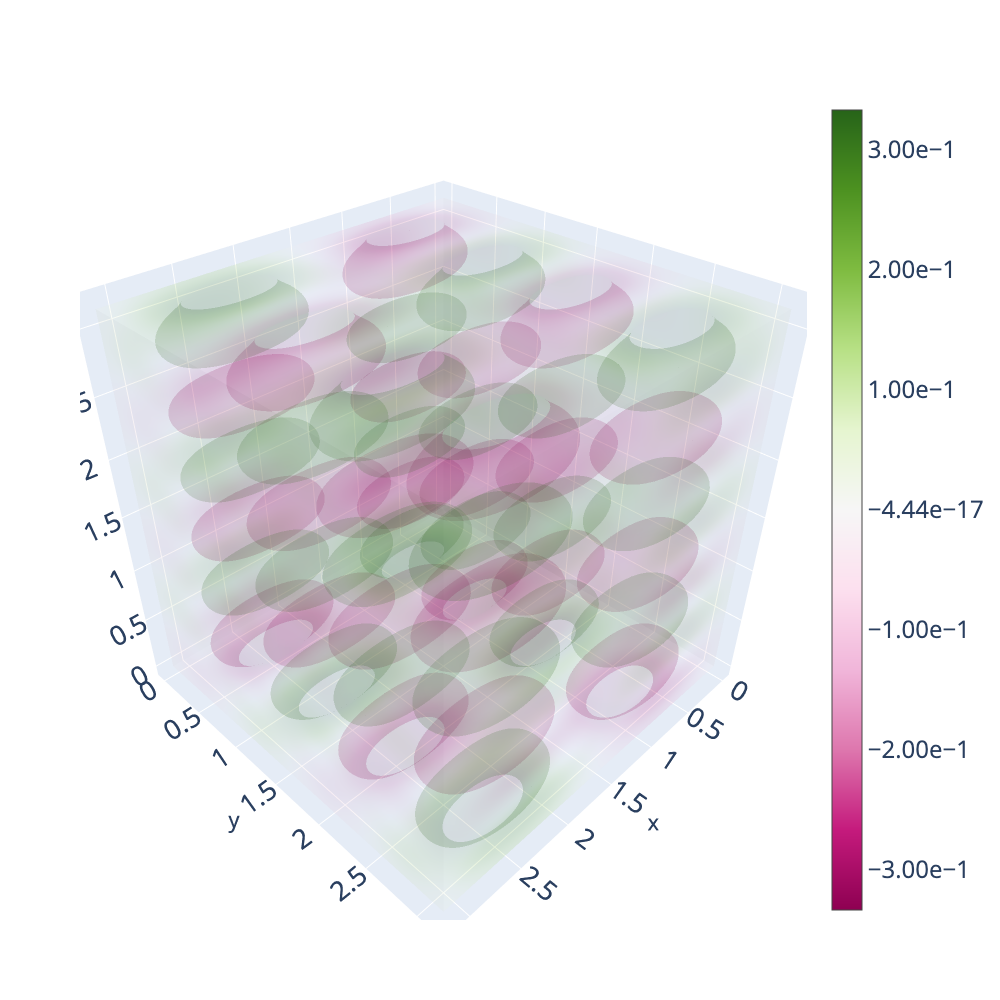
\includegraphics[width=\linewidth]{pictures/19_Lpi_128_analytical.png}
  \caption{$u_{analytical}$}
\end{subfigure}%
\begin{subfigure}{.33\textwidth}
  \centering
  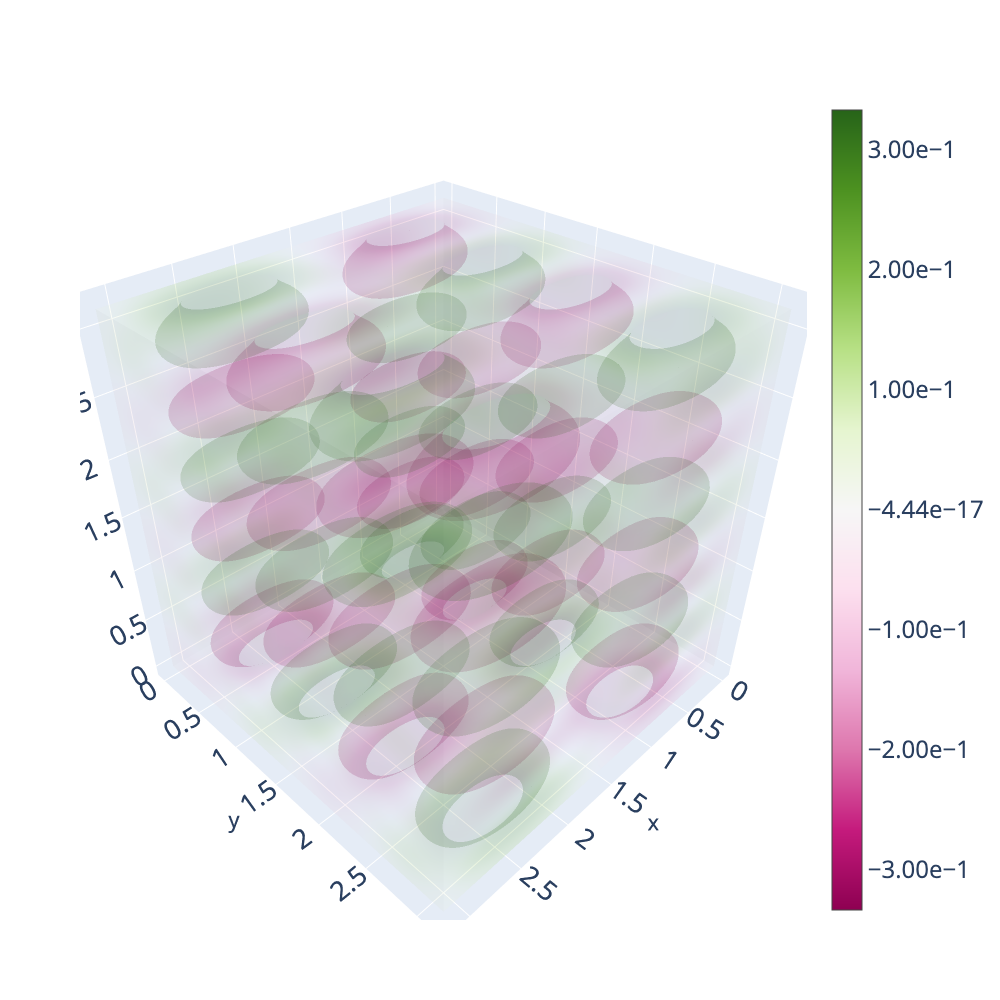
\includegraphics[width=\linewidth]{pictures/19_Lpi_128_calculated.png}
  \caption{$u_{calculated}$}
\end{subfigure}%
\begin{subfigure}{.33\textwidth}
  \centering
  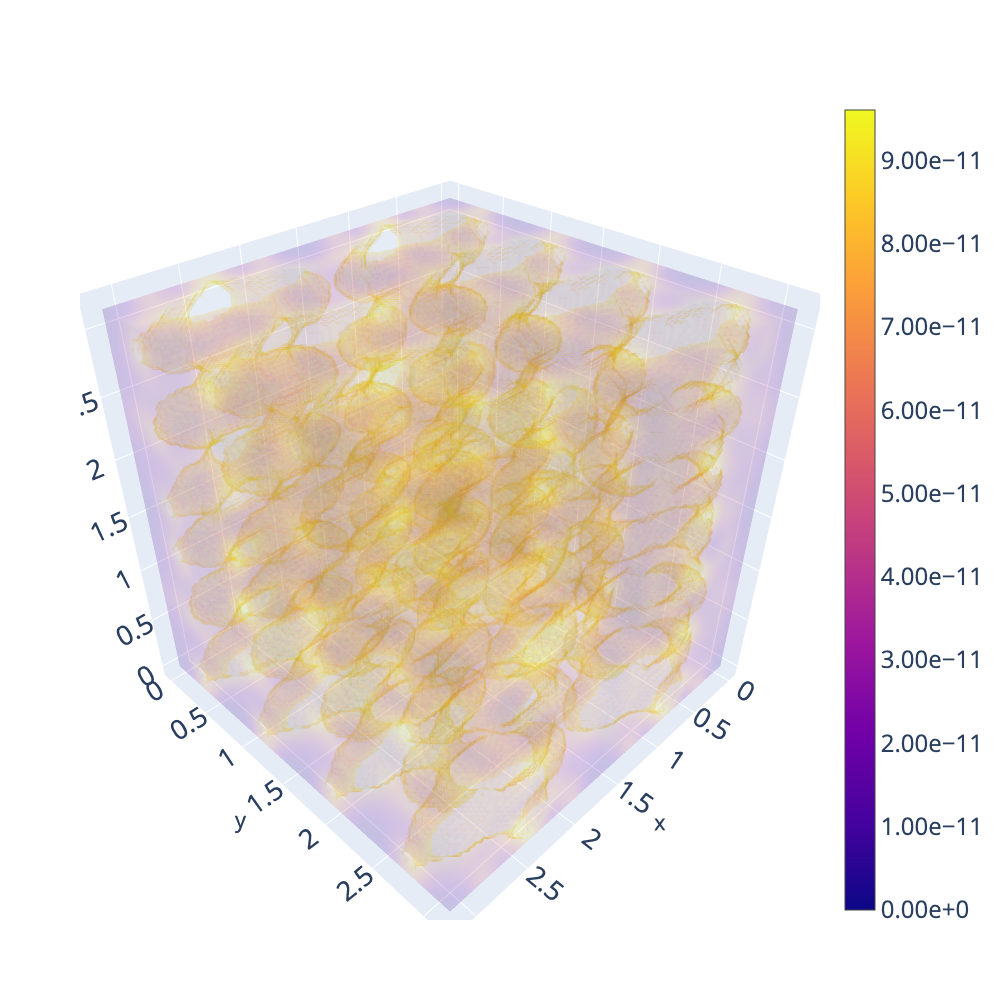
\includegraphics[width=\linewidth]{pictures/19_Lpi_128_diff.png}
  \caption{погрешность}
\end{subfigure}%
\caption{20 эпоха}
\label{fig:fig}
\end{figure}

\begin{figure}[H]
\begin{subfigure}{.5\textwidth}
  \centering
  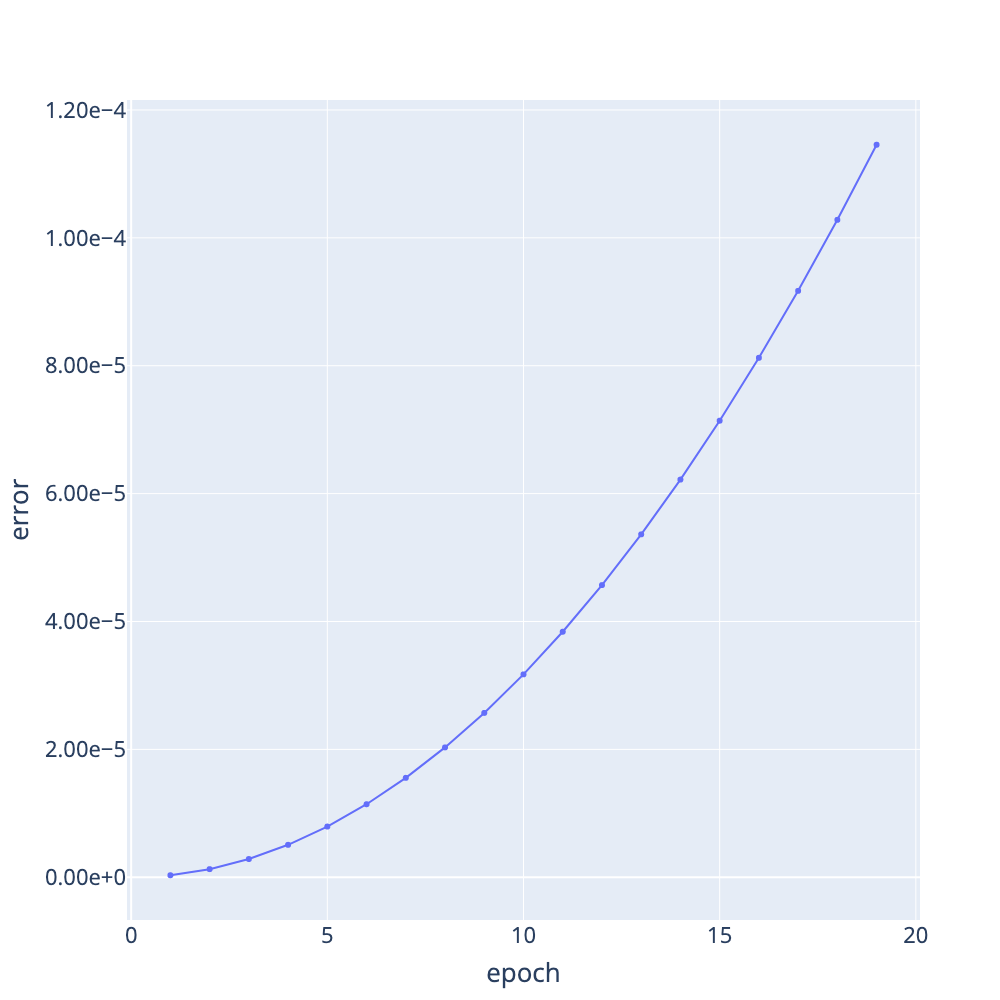
\includegraphics[width=\linewidth]{pictures/Lpi_128_errs.png}
  \caption{Погрешность от эпохи}
\end{subfigure}%
\begin{subfigure}{.5\textwidth}
  \centering
  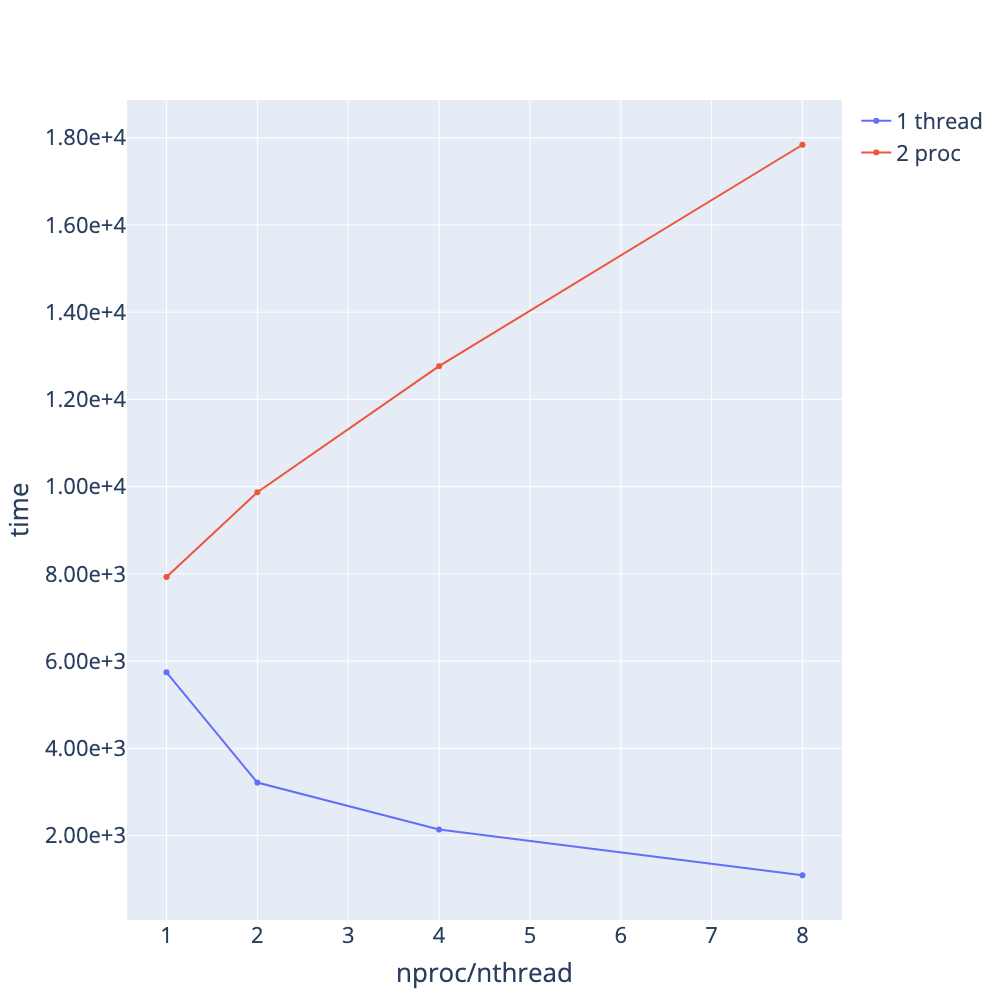
\includegraphics[width=\linewidth]{pictures/Lpi_128_perf.png}
  \caption{Время работы от конфигурации}
\end{subfigure}%
\end{figure}


\subsubsection{Графики для N=256}

\begin{figure}[H]
\begin{subfigure}{.33\textwidth}
  \centering
  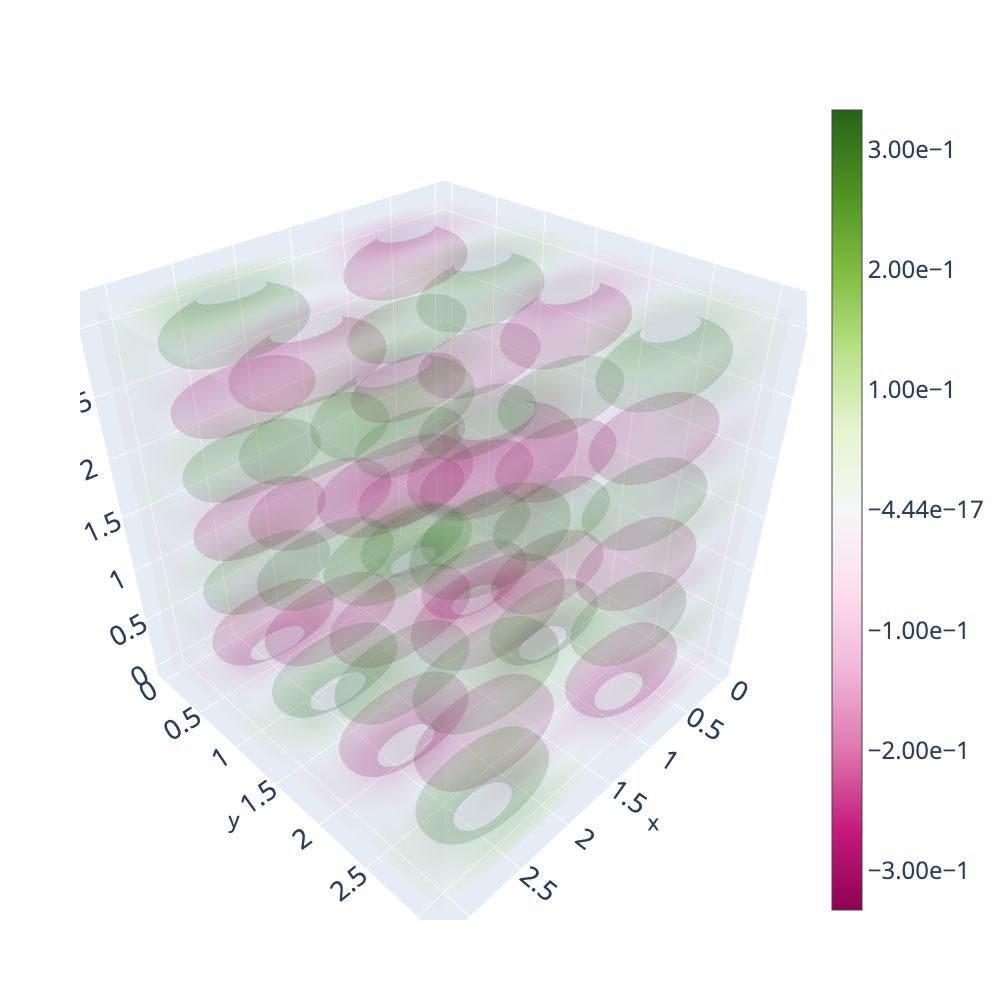
\includegraphics[width=\linewidth]{pictures/1_Lpi_256_analytical.png}
  \caption{$u_{analytical}$}
\end{subfigure}%
\begin{subfigure}{.33\textwidth}
  \centering
  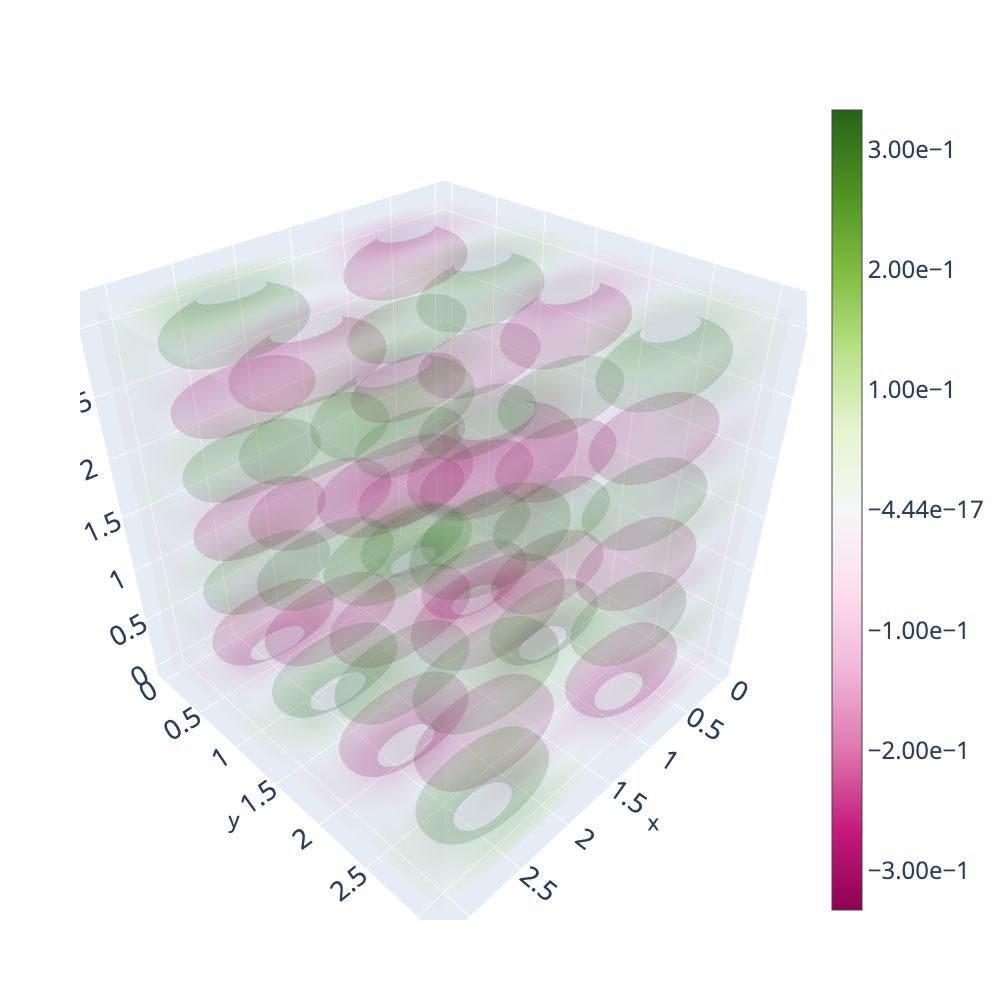
\includegraphics[width=\linewidth]{pictures/1_Lpi_256_calculated.png}
  \caption{$u_{calculated}$}
\end{subfigure}%
\begin{subfigure}{.33\textwidth}
  \centering
  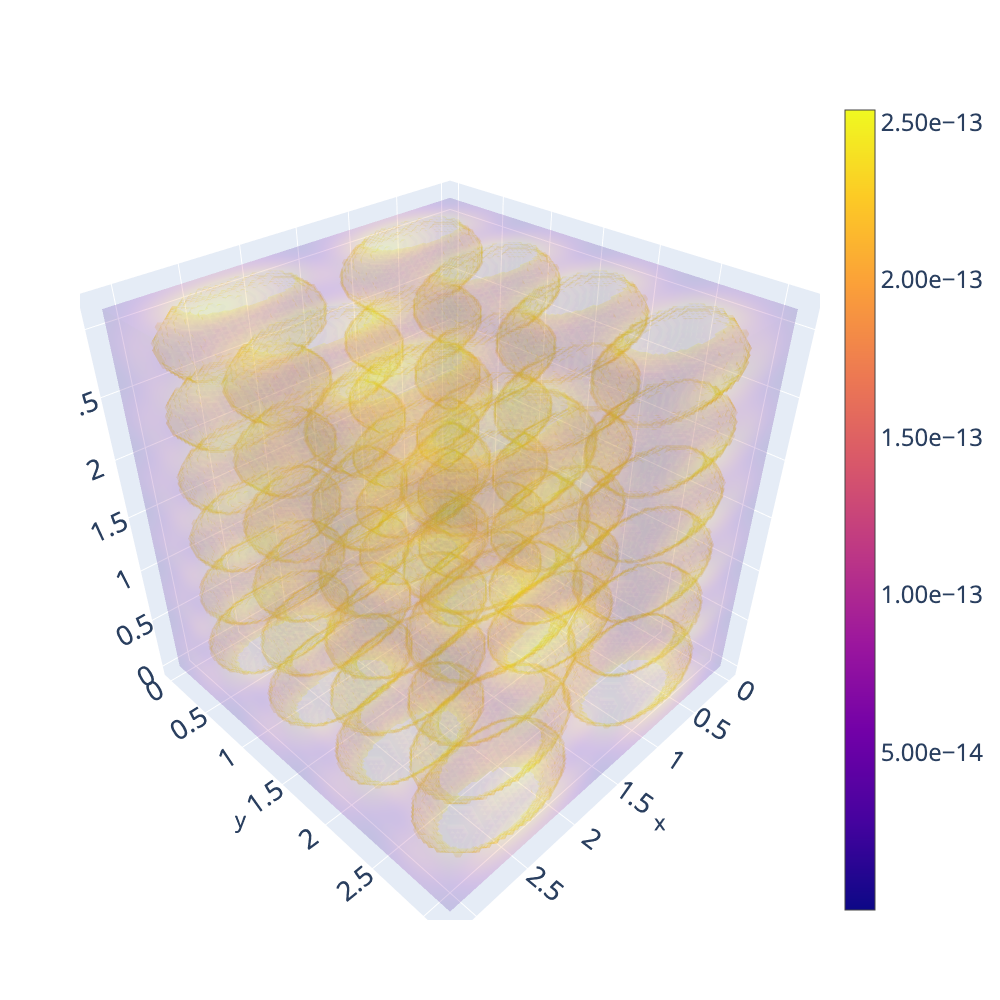
\includegraphics[width=\linewidth]{pictures/1_Lpi_256_diff.png}
  \caption{погрешность}
\end{subfigure}%
\caption{1 эпоха}
\label{fig:fig}
\end{figure}

\begin{figure}[H]
\begin{subfigure}{.33\textwidth}
  \centering
  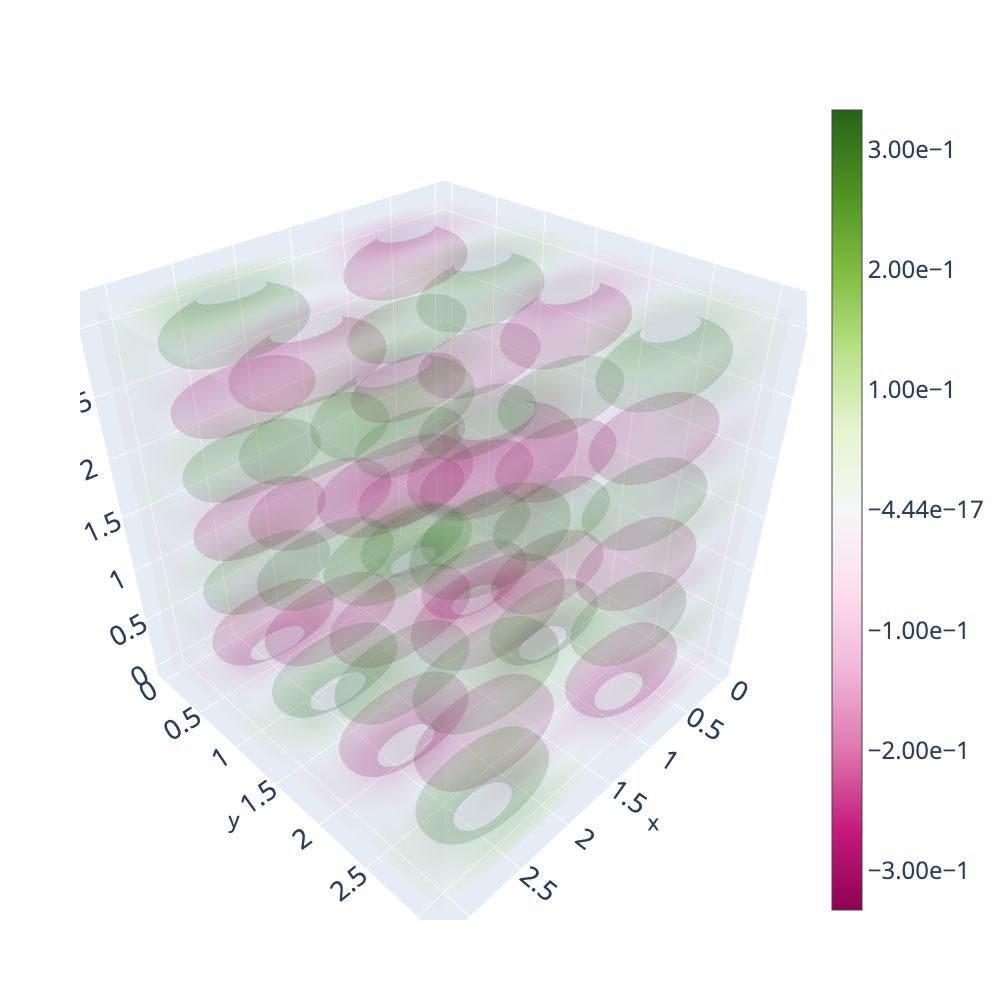
\includegraphics[width=\linewidth]{pictures/10_Lpi_256_analytical.png}
  \caption{$u_{analytical}$}
\end{subfigure}%
\begin{subfigure}{.33\textwidth}
  \centering
  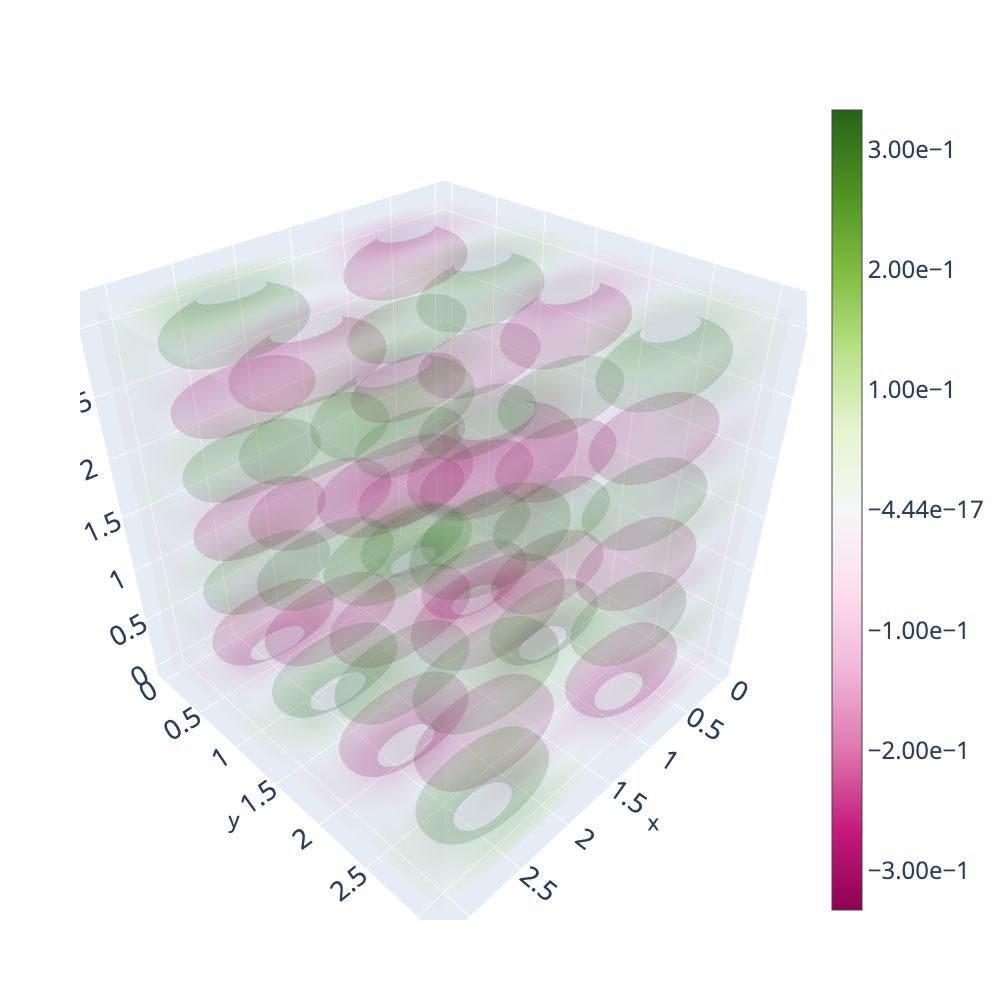
\includegraphics[width=\linewidth]{pictures/10_Lpi_256_calculated.png}
  \caption{$u_{calculated}$}
\end{subfigure}%
\begin{subfigure}{.33\textwidth}
  \centering
  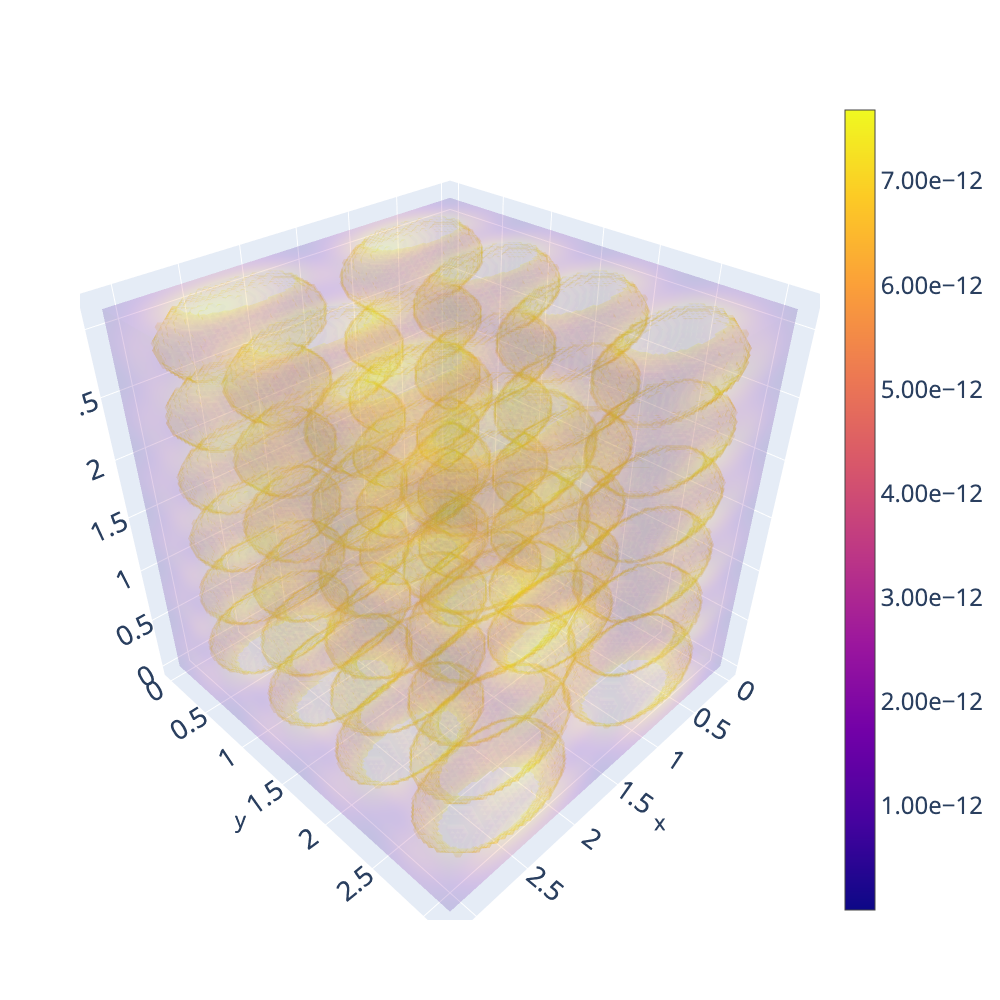
\includegraphics[width=\linewidth]{pictures/10_Lpi_256_diff.png}
  \caption{погрешность}
\end{subfigure}%
\caption{10 эпоха}
\label{fig:fig}
\end{figure}

\begin{figure}[H]
\begin{subfigure}{.33\textwidth}
  \centering
  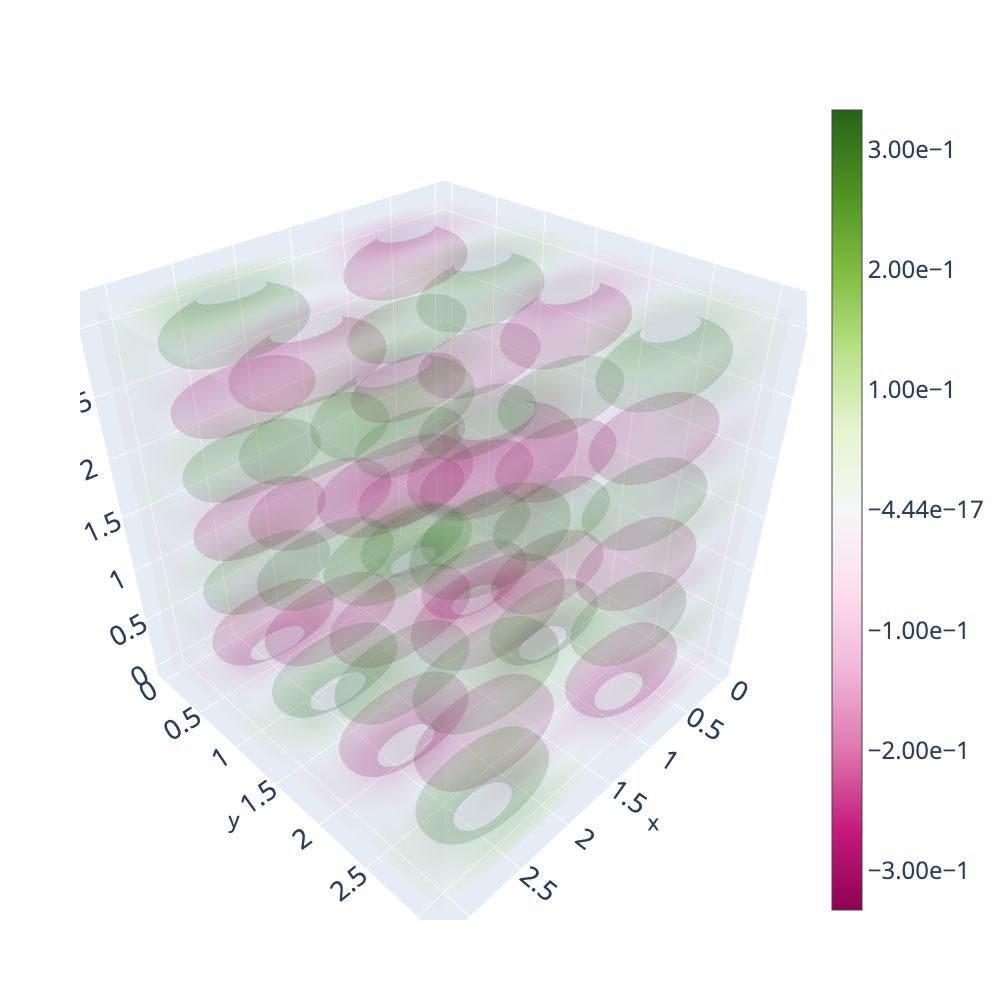
\includegraphics[width=\linewidth]{pictures/19_Lpi_256_analytical.png}
  \caption{$u_{analytical}$}
\end{subfigure}%
\begin{subfigure}{.33\textwidth}
  \centering
  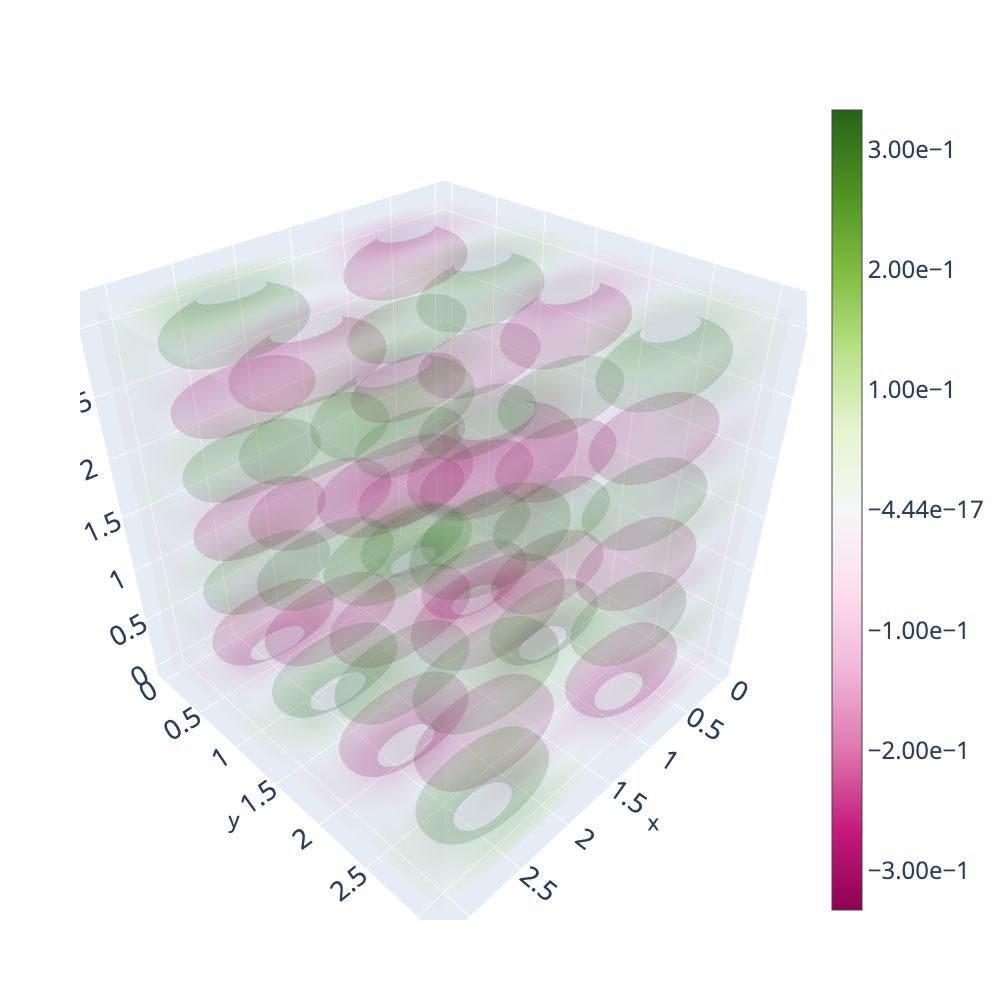
\includegraphics[width=\linewidth]{pictures/19_Lpi_256_calculated.png}
  \caption{$u_{calculated}$}
\end{subfigure}%
\begin{subfigure}{.33\textwidth}
  \centering
  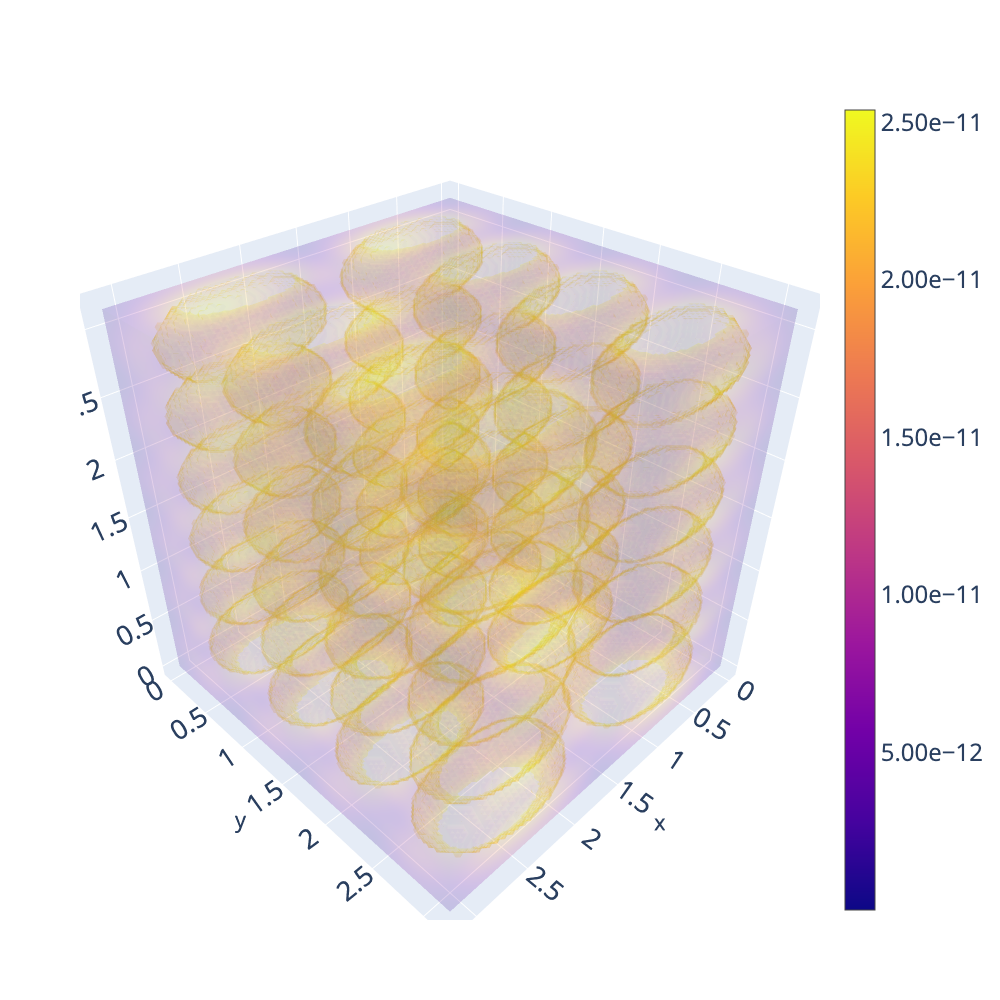
\includegraphics[width=\linewidth]{pictures/19_Lpi_256_diff.png}
  \caption{погрешность}
\end{subfigure}%
\caption{20 эпоха}
\label{fig:fig}
\end{figure}

\begin{figure}[H]
\begin{subfigure}{.5\textwidth}
  \centering
  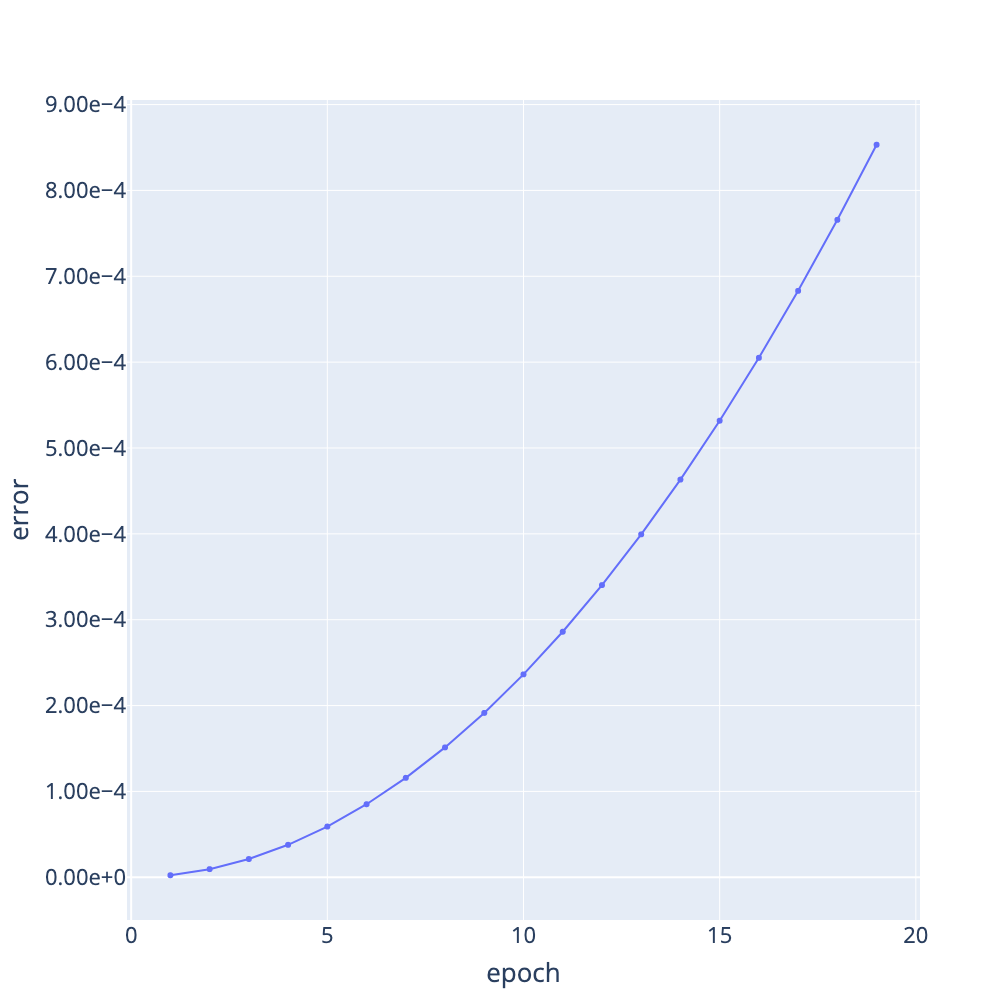
\includegraphics[width=\linewidth]{pictures/Lpi_256_errs.png}
  \caption{Погрешность от эпохи}
\end{subfigure}%
\begin{subfigure}{.5\textwidth}
  \centering
  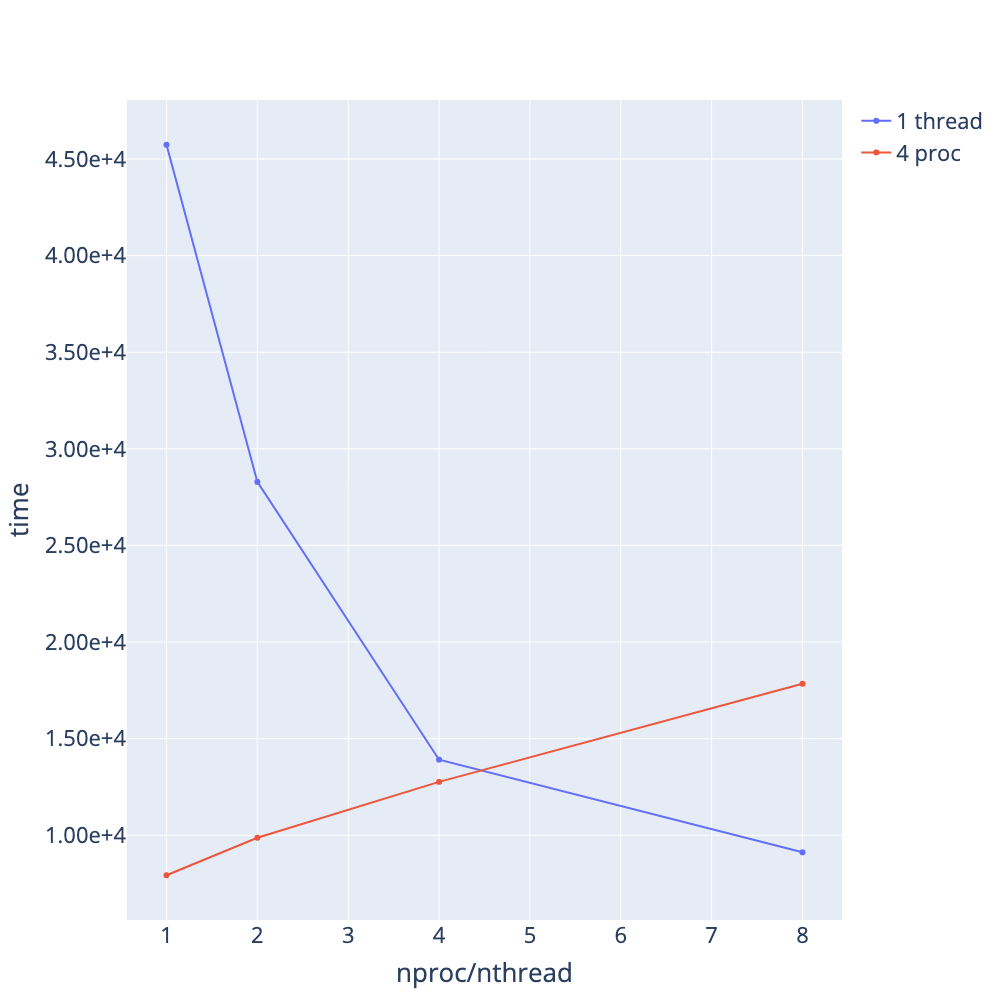
\includegraphics[width=\linewidth]{pictures/Lpi_256_perf.png}
  \caption{Время работы от конфигурации}
\end{subfigure}%
\end{figure}

\section{Заключение}

На основе анализа данных о запуске программы с различным числом процессов и на различных сетках можно сделать следующие выводы:

\begin{itemize}
    \item При запуске на суперкомпьютере рост производительности достигается только с ростом числа MPI процессов. Скорее всего, это связано с программным или аппаратным сбоем, мешающим работе гибридных программ.

    \item По графикам погрешности на обеих сетках (128, 256) хорошо видно, по какой функции расходится разностная схема. Вероятно, это говорит об отсутствии ошибок в программной реализации численного решения.
\end{itemize}
    

\end{document}
